\chapter{Lagrangian Method: Vortex Particle Method}
\label{ch:lagrangian}

	
%	\lsymb[f]{$\mathbf{x}$}{Position vector}{\si{\m}}{x}
%	\lsymb[f]{$\mathbf{x}_p$}{Position vector of the particle}{\si{\m}}{xp}
%	\lsymb[f]{$\mathbf{x}_{\nu}$}{Position vector of particle to be diffused}{\si{\m}}{xmm}
%	\lsymb[f]{$t$}{Time}{\si{\s}}{t}
%	\lsymb[f]{$\mathbf{u}$}{Velocity}{\si{\m\per\s}}{u}
%	%\lsymb[f]{$\mathbf{u}\left(\mathbf{x},t\right)$}{Velocity field}{$[m\cdot s^{-1}]$}{ua}
%	\lsymb[f]{$p$}{Pressure}{\si{\pascal}}{p}
%	\lsymb[f]{$\mathbf{u}^h$}{Discrete velocity}{\si{\m\per\s}}{uh}	
%	\lsymb[f]{$\mathbf{u}_{\infty}$}{Free-stream velocity}{\si{\m\per\s}}{ul}
%	\lsymb[f]{$\mathbf{u}_{\omega}$}{Vortical velocity}{\si{\m\per\s}}{uz}
%	\lsymb[f]{$\mathbf{u}_{\phi}$}{Potential velocity}{\si{\m\per\s}}{up}
%	\lsymb[f]{$\mathbf{u}_{\gamma}$}{Vortex sheet induced velocity}{\si{\m\per\s}}{uc}
%	\lsymb[f]{$\mathbf{u}_{\mathrm{ext}}$}{External induced velocity}{\si{\m\per\s}}{ue}
%	\lsymb[f]{$\mathbf{u}_{b}$}{Velocity of the body}{\si{\m\per\s}}{ub}	
%	\lsymb[f]{$\mathbf{u}_{\mathrm{slip}}$}{Boundary slip velocity}{\si{\m\per\s}}{us}	
%	\lsymb[f]{$u_{r}$}{Radial velocity}{\si{\m\per\s}}{ur}	
%	\lsymb[f]{$u_{\theta}$}{Angular velocity}{\si{\m\per\s}}{uhh}	
%
%		
%	\lsymb[f]{$N_p$}{Number of particles}{-}{np}	
%	\lsymb[f]{$\mathbf{K}$}{Biot-Savart kernel}{-}{k}
%	\lsymb[f]{$\mathbf{K_{\sigma}}$}{Vortex blob kernel}{-}{kb}	
%	\lsymb[f]{$h$}{Nominal particle spacing}{\si{m}}{h}	
%	\lsymb[f]{$\mathrm{overlap}$}{Overlap ratio of the blobs}{-}{o}	
%	\lsymb[f]{$W$}{Interpolation kernel weight}{-}{w}
%	\lsymb[f]{$\mathcal{E}$}{Enstrophy}{\si{m^2.s^{-2}}}{en}
%	\lsymb[f]{$c^2$}{Diffusion parameter}{-}{c}
%	\lsymb[f]{$\mathbf{\hat{n}}$}{Normal vector}{-}{n}
%	\lsymb[f]{$\mathbf{\hat{s}}$}{Tangent vector}{-}{s}	
%	\lsymb[f]{$h_{\nu}$}{Characteristic diffusion distance}{\si{m}}{hm}		
%	\lsymb[f]{$k_{d}$}{Diffusion frequency multiple}{-}{kd}			
%	
%	\lsymb[f]{$\mathbf{A}$}{Vortex panel influence matrix}{-}{kd}				
%
%	\lsymb[f]{$r$}{Radial position}{\si{m}}{r}
%
%	\gsymb[f]{$\zeta_{\sigma}$}{Smooth cut-off function of the blob}{-}{ff}	
%	\gsymb[f]{$\rho$}{Density}{\si{kg.m^{-3}}}{qq}
%	\gsymb[f]{$\nu$}{Kinematic viscosity}{\si{m^2.s^{-1}}}{mm}
%	\gsymb[f]{$\Gamma$}{Circulation}{\si{m^2.s^{-1}}}{c}
%	\gsymb[f]{$\Gamma_{\omega}$}{Circulation of the fluid}{\si{m^2.s^{-1}}}{cxx}	
%	\gsymb[f]{$\Gamma_{\gamma}$}{Circulation of vortex sheet}{\si{m^2.s^{-1}}}{ccc}		
%	\gsymb[f]{$\Gamma_{b}$}{Circulation of moving body}{\si{m^2.s^{-1}}}{cb}			
%	\gsymb[f]{$\omega$}{Vorticity}{\si{s^{-1}}}{xx}
%	\gsymb[f]{$\omega^h$}{Discrete vorticity field}{\si{s^{-1}}}{xxh}
%	\gsymb[f]{$\alpha_p$}{Circulation of the particle}{\si{m^2.s^{-1}}}{aap}
%	\gsymb[f]{$\beta_p$}{Corrected circulation of the particle}{\si{m^2.s^{-1}}}{bbp}
%	%\gsymb[f]{$\epsilon$}{Distance between the particles}{$[m]$}{eep}
%	\gsymb[f]{$\sigma$}{Core size}{\si{m}}{rr}
%	\gsymb[f]{$\Delta t_d$}{Diffusion time-step size}{\si{s}}{dtd}	
%	\gsymb[f]{$\Delta t_c$}{Convection time-step size}{\si{s}}{dtc}		
%	\gsymb[f]{$\gamma$}{Vortex sheet strengths}{\si{s}}{cc}		
%	\gsymb[f]{$\xi$}{Scale relative position of particle to stencil node}{-}{nn}
%	\gsymb[f]{$\epsilon$}{Relative error}{-}{ee}
%	\gsymb[f]{$\tau$}{Scaled viscous time}{\si{m^2}}{ss}
%	\gsymb[f]{$\Gamma_c$}{Circulation of the vortex core}{\si{m^2.s^{-1}}}{cc}

%To model the flow around a VAWT, several approaches can be taken, Vermeer at al. (2003) \cite{Vermeer2003} have also summarized in their paper. The two main approaches of investigating the flow is either employing a numerical method to simulate the flow or through experimental simulations.

%Leishman (2006) \cite{leishman2006principles} has shown that there are several simplified, efficient numerical tools that can be used to model the performance of a VAWT. Methods such as actuator disk theory and blade element momentum theory and deals with simplified Navier-Stokes equations and is very useful to evaluate the trend of certain design parameter. However, as they are highly simplified, complex flow phenomenons that has severe impact of the performance characteristics of the VAWT such as flow separation during dynamic stall, vortex shedding during the rotation and blade-wake interaction cannot be simulated. In order to understand them, either experimental investigation such as in wind tunnel or full Navier-Stokes simulations have to undertaken. So to understand the flow behaviour of a VAWT, several numerical research have been performed \cite{Almohammadi2013} \cite{Ferreira2007} \cite{Islam2008} \cite{Merz2012} and experimental researches by Ferreira \cite{SimaoFerreira2008} \cite{Ferreira} and others \cite{Howell2010} \cite{Mertens2003}.
%\index{Actuator disk}

%All the numerical method that was grid-based struggled with dealing with large number of mesh cells for high Reynolds numbers and the numerical method that employed simplified Navier-Stokes methods had to sacrifices some accuracies.The experimental investigation also come with drawbacks as they are require more financial resources and usually only feasible to model the scaled VAWTs.

%This is the main relevance of the hybrid vortex particle method for the VAWT investigations. By utilizing the two methods together, the vortex particle method away from body, and Navier-Stokes solver with turbulence model in the near-body region, one will be able to tackle the challenges in an efficient manner.

%Therefore, this chapter is dedicated to given an overview on the theory of the Vortex Particle Method which we will employ with coupled Navier-Stokes solver. 

%------------------------------------------------------------------------------------------------------
%------------------------------------------------------------------------------------------------------
%------------------------------------------------------------------------------------------------------
\section{Introduction to the Vortex Particle Method}
\label{sec:introtovpm}
\indexAcron{Vortex Particle Method}{VPM} is a numerical method employed in computational fluid dynamics, dealing with the evolution of the vorticity in the fluid from a Lagrangian description. In an Eulerian formulation, the fluid is viewed at a fixed window where the change in the fluid properties are evaluated. However, the Lagrangian formulation, regards the fluid as a collection of particles (or elements) carrying properties of the fluid (such as vorticity, mass, etc.). 

Efficient discretization of the fluid domain becomes a difficult task for cases such as \printAcron{Vertical-Axis Wind Turbine}{VAWT}, where the wake geometry is complex and unsteady. Discretizing such wake using Eulerian formulation becomes difficult as it requires the adaption of the mesh over time for efficient computation. The VPM only needs fluid elements where there is vorticity meaning that the method is inherently auto-adaptive. This is one of the advantage of the VPM. Furthermore, with computational acceleration methods such as \printAcron{Fast-Multipole Method}{FMM} and parallel computation in \printAcron{Graphics Processing Units}{GPU} enables an efficient evolution of the vorticity wake. 

However, the key advantage of the VPM is that it is ideal for capturing the resolving the long-time characteristics of the unsteady compact vortical structures that are shed off from the VAWT blades, as described by Stock \cite{Stock2010a}, providing the motivation for using VPM for modeling the rotor wake.

A summary of the advantage of the Lagrangian vortex method w.r.t the Eulerian method was provided by Wee and Ghoniem \cite{Wee2006a}:
\begin{itemize}
\item Eulerian methods introduce dissipation, even in flows with zero velocity gradient. However such error as minimized at the convection of the Lagrangian method.
\item The numerical stability of the Lagrangian method is not restricted by the CFL condition.
\item The support of the Lagrangian elements are a small fraction of the fluid domain. The support is confined to location of non-zero vorticity, making the method naturally grid adaptive.
\end{itemize}

The main literature on the VPM (the Lagrangian component of the hybrid method), is the book of Cottet and Koumoutsakos, Vortex Methods: Theory and Practice \cite{Cottet2000a}. It gives an insight on the fundamentals of the vortex method (specifically VPM) and gives a summary on hybrid methods.

\subsection{Vorticity}
The vorticity $\omega$ is the governing element of the VPM. It is given by
	\begin{equation}
	\mathbf{\omega} = \nabla \times \mathbf{u},
	\label{eq:lag_vort}
	\end{equation}
where $\mathbf{u}$ is the velocity vector field. In 2D, the circulation $\Gamma$ is defined by Stokes' theorem as,

	\begin{equation}
	\Gamma = \int_L\mathbf{u}\cdot \mathrm{d}s= \int_A (\nabla \times \mathbf{u}) \cdot \mathbf{n}\ \mathrm{d}A = \int_A\omega\cdot\mathbf{n}\ \mathrm{d}A,
	\label{eq:definitionOfCirculation}
	\end{equation}

and represents the flux integral of vorticity across the surface $A$, contoured by the line $s$. Figure \ref{fig:vorticityCirculation} depicts this relation of velocity $\mathbf{u}$, vorticity $\omega$ and the circulation $\Gamma$.

	\begin{figure}[!h]
	\centering
	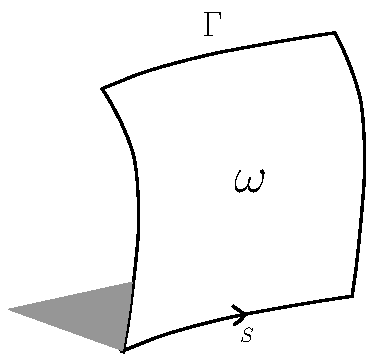
\includegraphics[width=0.3\linewidth]{./figures/lagrangian/vorticityCirculation_updated.pdf}
	\caption{Definition of the circulation in the fluid.}
	\label{fig:vorticityCirculation}
	\end{figure}

 
\subsection{Velocity-Vorticity formulation of the Navier-Stokes equations}
The governing equation of the vortex particle method is the velocity-vorticity formulation $\mathbf{u}-\omega$ of the Navier-Stokes equations, as presented in Cottet and Koumoutsakos \cite{Cottet2000a}. It is derived from the 2D incompressible Navier-Stokes momentum equation, given as,
	\begin{equation}
	\frac{\partial \mathbf{u}}{\partial t} + \mathbf{u}\cdot\nabla\mathbf{u} = - \frac{1}{\rho} \nabla p + \nu \nabla^2\mathbf{u},
	\label{eq:mom}
	\end{equation}
relating the velocity field $\mathbf{u}\left(\mathbf{x},t\right)$ to the pressure field $p\left(\mathbf{x},t\right)$, the kinematic viscosity $\nu$ and density $\rho$, and satisfied the incompressibility constraint,
	\begin{equation}
	\nabla\cdot\mathbf{u} = 0,
	\label{eq:la_ic}
	\end{equation}
The curl of the equation \ref{eq:mom} is take to obtain the velocity-vorticity formulation, 
	\begin{equation}
	\frac{\partial \omega}{\partial t} + \mathbf{u}\cdot\nabla\omega = \nu \nabla^2 \omega,
	\label{eq:la_vteq}
	\end{equation}
relating the vorticity $\omega$ to the velocity $\mathbf{u}$. Note that the pressure term $p$ disappear  from the equality.

\subsection{Viscous splitting algorithm}
\label{subsec:vsa}
The VPM was initially used to model the evolution of incompressible, inviscid flows. However, in order to simulate a real flow, we must also deal with the viscous behavior of the fluid. Chorin in 1973 \cite{Chorin1973a}, showed that using the viscous splitting algorithm, it is possible to take the viscous effects of the flow into account. 

The viscous splitting algorithm is a fractional step method, where the viscous and the inviscid part of the vorticity transport equation, equation \ref{eq:la_vteq}, are dealt with in two subsequent sub-steps,

	\begin{enumerate}
	\item \textbf{Convection} (sub-step 1):
		\begin{equation}
		\frac{\partial\omega}{\partial t} + \mathbf{u}\cdot\nabla\omega=0;
		\label{eq:convectionEulerian}
		\end{equation}
		
	\item \textbf{Diffusion} (sub-step 2):
		\begin{equation}
		\frac{\partial\omega}{\partial t} = \nu\nabla^2\omega.
		\label{eq:vsa2}
		\end{equation}
	\end{enumerate}

The first sub-step of the evolution deals with the convection of vorticity. The convection step is described in section \ref{sec:covb}. The diffusion of vorticity field is dealt with in the second sub-step. The diffusion of the vorticity field is dealt with in section \ref{sec:diffusionVM}

%There are many ways of treating the diffusion of the vorticity field. In this work, we initially used the modified interpolation kernel by Wee (2006) \cite{Wee2006a} that simultaneously discretizes diffusion and redistributes the vortex particles. Later, we used a simple redistribution scheme of Tutty (2010) \cite{Tutty2010a}, that did not constraint the minimum time-step size, see section \ref{sec:diffusionVM}.

%------------------------------------------------------------------------------------------------------
%------------------------------------------------------------------------------------------------------
%------------------------------------------------------------------------------------------------------
\section{Spatial discretization: Introduction to vortex blobs}
\label{sec:spatialDiscretization}

The vorticity $\omega$ and the velocity $\mathbf{u}$ in the vorticity transport equation, equation \ref{eq:la_vteq}, describes a continuous field. However, these variables needs to be discretized to perform a numerical integration required for the numerical simulation. 

\subsection{Discrete form of vorticity field}
\label{subsec:discreteVorticity}
The vorticity field is discretized by representing the continuous vorticity field by a summation of particle-type elements, as described by Barba \cite{Barba2010a}. The discrete vorticity field $\omega^h$ is represented by a linear combination of $N$ basis function, given as,
	\begin{equation}
	\omega\left(\mathbf{x},t\right) \simeq \omega^h\left(\mathbf{x},t\right) = \sum_{p}^N\alpha_p\left(t\right)\delta \left[\mathbf{x}-\mathbf{x}_p\left(t\right)\right],
	\end{equation}
where $\delta$ is the Dirac delta function, and $\alpha_{p}$ is the circulation carried by the particle at $\mathbf{x}_p$. We must note that $\omega^h$ is the discrete vorticity field and therefore in an approximation of the continuous vorticity field $\omega$. 

The velocity $\mathbf{u}$ is related to the vorticity $\omega$ using the Biot-Savart Law.

\subsection{Biot-Savart Law}
A velocity field $\mathbf{u}$ that satisfies the incompressibility constraint, equation \ref{eq:la_ic}, can be decomposed using the Helmholtz decomposition,
	\begin{equation}
	\mathbf{u} = \mathbf{u}_{\omega} + \mathbf{u}_{\phi} + \mathbf{u}_{\delta},
	\label{eq:helmholtz}
	\end{equation}
where $\mathbf{u}_{\omega}$ is the rotational (solenoidal) component of the velocity $\mathbf{u}$, $\mathbf{u}_{\phi}$ is the irrotational (potential) component, and $\mathbf{u}_{\delta}$ is the harmonic form. These components satisfying the following equality,
	\begin{equation}
	\nabla \cdot \mathbf{u}_{\omega} = \nabla \times \mathbf{u}_{\phi} = \nabla^2\mathbf{u}_{\delta} = 0.
	\end{equation}
 
The divergence-free component $\mathbf{u}_{\omega}$ implies that there exists a stream function $\psi$, such that,
	\begin{equation}
	\mathbf{u}_{\omega} = \nabla \times \psi,
	\end{equation} 
and therefore the vorticity $\omega$ of the velocity $\mathbf{u}$, is given as,
	\begin{equation}
	\omega = \nabla \times \mathbf{u} = - \Delta \psi
	\label{eq:la_vorPois}
	\end{equation}

Similarly, there must exist a potential $\phi$, such that,
	\begin{equation}
	\mathbf{u}_{\phi} = \nabla \phi.
	\end{equation}
For an incompressible and unbounded problem, the potential velocity $\mathbf{u}_{\phi}$ is simply the free-stream velocity $\mathbf{u}_{\infty}$ and the harmonic form $\mathbf{u}_b = 0$. In the case of the bounded problem with solid boundaries, the presence of the body must be taken into account, see section \ref{sec:boundaryConditions}. For now, we will discuss the unbounded problem.

From the Poisson equation \ref{eq:la_vorPois}, the velocity is related to the vorticity by the Biot-Savart law, given as,
	\begin{equation}
	\mathbf{u}_{\omega} = \mathbf{K}\star\omega,
	\end{equation}
where $\star$ is the convolution of the vorticity with the 2-D Biot-Savart kernel $\mathbf{K}$ given by,
	\begin{equation}
	\mathbf{K} = \frac{1}{2\pi\left|\mathbf{x}\right|^2}\left(-x_2,x_1\right).
	\label{eq:GreensKernel}
	\end{equation}
From the kernel, we see that as the distance to the kernel center approaches zero ($\mathbf{x} \rightarrow 0$), the kernel goes to infinity. The singularity of the kernel $\mathbf{K}$ is removed by mollifying the kernel distribution ensuring smooth velocity distribution.

%Thus the discrete vorticity field is an $N$-body problem inducing velocity on each other. So, to evolve the vorticity field, we simply have to evolve the vortex particles with the induced velocity acting on it. This is the main advantage of the vortex particle method as there are efficient methods to evaluate the induced velocities. The $N$-body problem can be parallelized in GPUs, and furthermore the induced velocity calculations can be simplified using fast summation methods such as the \printAcron{Fast Multipole Method}{FMM}, reducing the problem from $\mathcal{O}(N^2)$ to $\mathcal{O}(N)$, in an ideal case.


\subsection{Mollified vortex kernels}
\label{subsec:mvk}
A mollified (or a regularized) vortex particle is called the vortex blob, and has a non-zero vortex core size $\sigma$. A smoothing function $\zeta$ is used to mollify the kernel $\mathbf{K}$, satisfying the constraint $\int \zeta = 1$, such that the circulation is conserved. An ideal choice for a smoothing function is the Gaussian distribution, given as,
	\begin{equation}
	\zeta_{\sigma} = \frac{1}{k\pi\sigma^2}\exp\left(-\frac{\left|\mathbf{x}\right|}{k\sigma^2}\right),
	\end{equation}

where typically $k$ is either 1, 2 or 4, determining the width of the kernel, and $\sigma$ being the core-size of the vortex blob.
	\begin{figure}[!h]
	\centering
	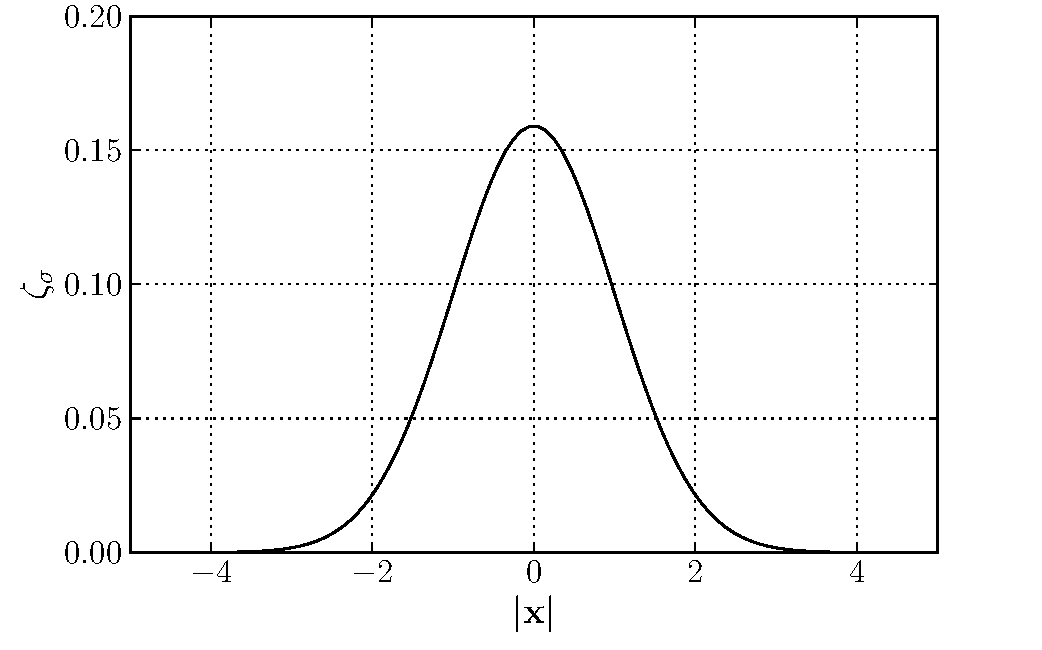
\includegraphics[width=0.6\textwidth]{figures/lagrangian/gaussianKernel.pdf}
	\caption{The smoothing function $\zeta_{\sigma}$ for a gaussian distribution with $k=2$, $\sigma=1$.}
	\label{fig:gaussianDistribution}
	\end{figure}

Figure \ref{fig:gaussianDistribution} depicts the smoothing function $\zeta_{\sigma}$ with $k=2$ and $\sigma = 1$, showing that the function decays quickly away from the center of the core. The mollified Biot-Savart kernel $\mathbf{K}_{\sigma}$ is given as,	 
	\begin{equation}
	\mathbf{K}_{\sigma} = \mathbf{K} \star \zeta_{\sigma}, 
	\end{equation}
resulting in the discrete mollified vorticity field as,
	\begin{equation}
	\omega^h\left(\mathbf{x},t\right) = \sum_p \alpha_p\left(t\right)\zeta_{\sigma}\left[\mathbf{x}-\mathbf{x}_p\left(t\right)\right],
	\label{eq:mollifiedVorticityField}
	\end{equation}
and the discrete mollified velocity field as,
	\begin{equation}
	\mathbf{u}^h\left(\mathbf{x},t\right) = \sum_p \mathbf{K}_{\sigma}\left[\mathbf{x}-\mathbf{x}_p\left(t\right)\right]\alpha_p\left(t\right).
	\label{eq:mollifiedVelocityField}	
	\end{equation}

Koumoutsakos and Chorin \cite{Cottet2000a}, explained that in order to ensure the smoothness of the velocity field, the vortex blobs need to have an overlap with each other. The overlap ratio $\lambda$ is defined as,
	\begin{equation}
	\lambda = \frac{h}{\sigma},
	\label{eq:overlapRatio}
	\end{equation}
where $h$ is the nominal particle spacing, and $\sigma$ is the vortex blob core size. Figure \ref{fig:blobOverlap} shows the visual representation of this definition. 

The overlap constraint is violated during the convection of the vortex blobs. Due to the strains in the flow, the vortex blobs cluster together at certain regions and disperse at others. This localized clustering effect is seen as a Lagrangian grid distortion, which is dealt with using a remeshing technique, section \ref{subsec:remeshing}.

	\begin{figure}[!t]
	\centering
	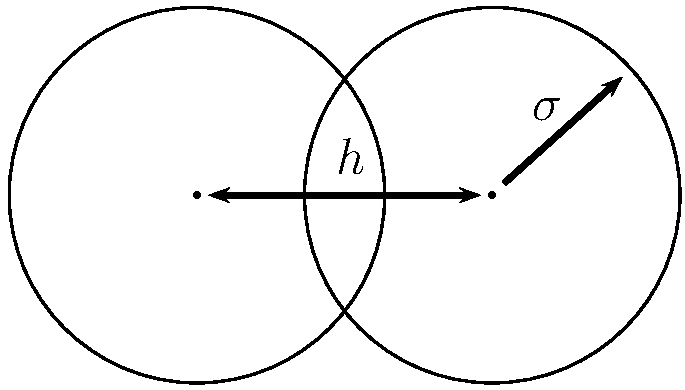
\includegraphics[width=0.4\textwidth]{figures/lagrangian/blobOverlap.pdf}
	\caption{Vortex blob with an overlap ratio $\lambda = h/\sigma$}
	\label{fig:blobOverlap}
	\end{figure}

\subsection{Vortex blob initialization}
\label{subsec:vortexBlobInitialization}
Now the question arises on how should we initialize the particle's circulation strengths $\alpha_p$ of equation 	\ref{eq:mollifiedVorticityField}. The common approach, that is used as a standard, is to estimate the particles strength by quadrature,
	\begin{equation}
	\alpha_p = \omega_p\cdot h^2,
	\label{eq:particleCirculationAssignment}
	\end{equation}

	\begin{figure}[!b]
	\centering
	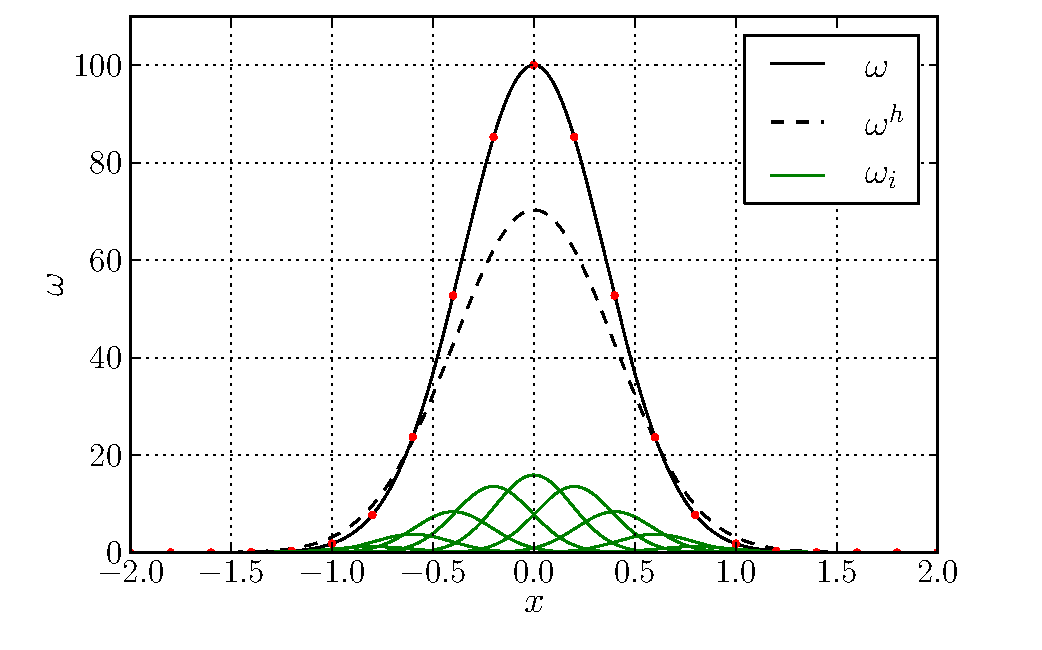
\includegraphics[width=0.6\textwidth]{figures/lagrangian/particleInitialization.pdf}
	\caption{Mollified vorticity field of a Gaussian vorticity distribution by blobs with $\lambda=1.0$, $\sigma=0.19$, and $h=0.19$. Vortex blob strengths were assigned using equation \ref{eq:particleCirculationAssignment}, sampling the exact vorticity [{\color{plotRed}{$\bullet$}}, {\color{plotRed}{\textbf{red}}} dot]. Figure depicts the exact vorticity distribution $\omega$ [---, solid \textbf{black}], the vorticity distribution of each blob $\omega_i$ [{\color{darkgreen}{---}}, solid {\color{plotGreen}{\textbf{green}}}], and the mollified vorticity field from the blobs $\omega^h$ [- -, dashed \textbf{black}].  }
	\label{fig:particleInitialization}
	\end{figure}

meaning that the particle carries the circulation of its local area. This might seem like a valid assumption as the circulation of a given area is the integral of the vorticity in the area, given by equation\ \ref{eq:definitionOfCirculation}, and therefore we will be conserving the circulation as all the circulation in the fluid is represented by the blobs.

Figure \ref{fig:particleInitialization} shows the initialization of the vorticity field using the equation 	\ref{eq:particleCirculationAssignment}. We observed that the mollified vorticity field $\omega^h$, deviates from the original intended vorticity distribution $\omega$. Barba and Rossi \cite{Barba2010a}, have described this problem as Gaussian blurring of the original vorticity field due to use of mollified vortex kernel $\zeta_{\sigma}$ in equation 	\ref{eq:mollifiedVorticityField}. Even though the total circulation is conserved, locally we see that the circulation is not conserved. 

This phenomenon causes issue during the coupling of the Lagrangian method and the Eulerian method, as particle in the overlap region are re-initialized at every step of the hybrid method. This error in initialization posses a challenge in the coupling of the method and is described in section \ref{subsec:hy_iwtca}.

A typical strategy for recovering the intended distribution is the Beale's Iterative Method \cite{Beale1988}, as used by Koumoutsakos and Cottet \cite{Cottet2000a}. The method is particle circulation processing scheme where the circulation $\alpha_p$ of the particles are modified iteratively such that the mollified vorticity field $\omega^h$ matches the original distribution $\omega$. However, the Beale's method required the correction of complete vorticity field in fluid domain and cannot be used to correct only part of the fluid domain, as required for our decomposed domain method. Therefore, an alternate method is required to minimized the error in particle initialization.

%################# Beale's Iterative method, removed.
\begin{comment}
Another way of viewing this phenomenon is to say that the conservation of circulation is only valid globally (for an infinite domain), but once we try to conserve circulation locally (e.g. in a given sub-domain), is does not satisfy anymore. Figure \ref{fig:particleInitialization} shows this effect for a simple gaussian initial vorticity distribution $\omega$. The mollified vorticity field is given as $\omega^h$ and even though the integral of both function is the same (conservation of circulation is satisfied), the vorticity functions do not match. This is does not cause a lot of issues when we only dealing with vortex particle method, however once we start using domain decomposition methods, this problem is an issue. As the vorticity is the communication between both methods, we must have accurate vorticity distribution.

A common strategy, used by Koumoutsakos, Cottet, and other for recovering the initial vorticity field is to perform the Beale's method \cite{Beale1988} \cite{Cottet2000a}.


\subsubsection*{Beale's Iterative Method}
\label{subsubsec:BealesMethod}
The Beale's method is particle circulation processing scheme where the circulation of the particles are modified such that the mollified vorticity field matches the indented vorticity field (the initial vorticity field). The recovery of the vorticity field is done by performing a discrete deconvolution,
	\begin{equation}
	\sum_j^N \beta_j \zeta_{\sigma}\left(\mathbf{x}_i-\mathbf{x}_j\right) = \omega_i,
		\end{equation}
where $\beta_j$ is the circulation of the particles at positions $\mathbf{x}_j$ such that it matches the exact vorticity $\omega_i$ at the position $\mathbf{x}_i$ that we are evaluating.  As we are try to solve for a $N$ unknown problem, we must set up an $N$ system of equations. Multiplying both sides with the area associated to the blobs, we get
	\begin{equation}
	\mathbf{A}_{ij} \beta_j = \alpha_i^{\mathrm{exact}},
	\end{equation}
where
	\begin{equation}
	\mathbf{A}_{ij} = \zeta_{\sigma}\left(\mathbf{x}_i - \mathbf{x}_j\right) \cdot h^2.
	\end{equation}

This is an $N \times N$ matrix containing the weights of the influence of each particle on each other. When we are dealing with large number of vortex blobs, we see that it is very expensive to invert the matrix $\mathbf{A}$, meaning that we would have to use a more efficient method. Furthermore as the deconvolution problem is a severely ill-condition problem \cite{Cottet2000a}, we should not directly invert the matrix. Beale's proposition to this problem was to iteratively solve for the solution,
	\begin{equation}
	\beta_{j}^{n+1} = \alpha_i + \beta_i^n - \mathbf{A}_{ij}\cdot\beta_j^n
	\end{equation}
	
We see that with just two iterations, the error between the mollified and exact vorticity field reduces drastically, figure \ref{fig:bealesCorrection}. Koumoutsakos and Cottet \cite{Cottet2000a}, had shown that there was a drastic improvement in the velocity with just two to three iterations. However, the average vorticity of the blobs cell $\tilde{\omega} = \beta/h^2$ (red dot in figure \ref{fig:bealesCorrection}), is more peaky and no longer matches the initial vorticity distribution. This means that if we try to fix the mollified vorticity distribution to match the correct initial vorticity distribution, we corrupt the local circulation even more.

The another downside of using the Beale's correction method that it is only valid for an infinite domain as it performs a discrete deconvolution of a gaussian kernel with an infinite span. Therefore it applies to all of the fluid domain, meaning that if we are dealing with a decomposed domain with finite bounds, the Beale's correction cannot be used and would result in spurious results. So the Beale's correction can and should only be used for correcting the vorticity field of the whole fluid domain.

	\begin{figure}[t]
	\centering
	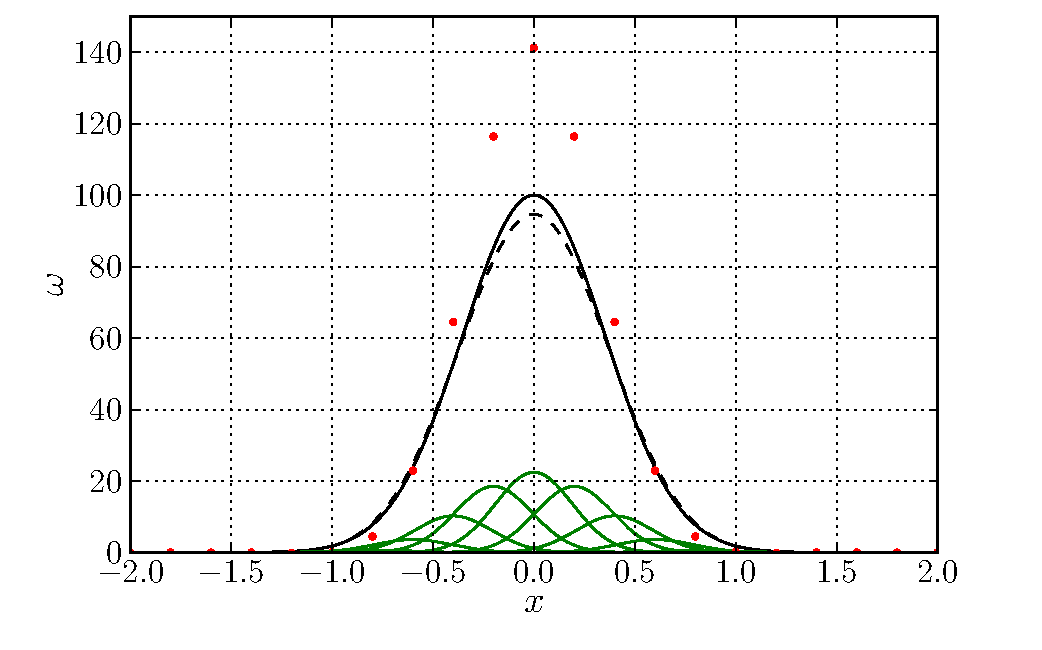
\includegraphics[width=0.7\textwidth]{figures/lagrangian/bealesCorrection.pdf}
	\caption{Mollified vorticity field after two Beale's iteration, with $\mathrm{overlap}=1.0$, $\sigma=0.19$, $h=0.19$. Figure depicts exact vorticity distribution $\omega$ [---, solid black], vorticity distribution of each blob $\omega_i$ [{\color{plotGreen}{---}}, dashed green], the mollified vorticity field $\omega^h$ [- -, dashed black], and the corrected blob cell vorticity $\tilde{\omega}=\beta/h^2$ [{\color{plotRed}{$\bullet$}}, red dot].}
	\label{fig:bealesCorrection}
	\end{figure}
\end{comment}


\subsection{Minimization of particle discretization error}
\label{subsubsec:convergenceInterpolation}
An alternate method to reduce the Gaussian blurring of the vorticity field is to modify the overlap ratio $\lambda$, and the nominal particle spacing $h$. This approach does not remove the Gaussian blurring problem, but instead minimizes its discretization error.
	
\begin{figure}[!b]
        \centering
        \begin{subfigure}[b]{0.5\textwidth}
                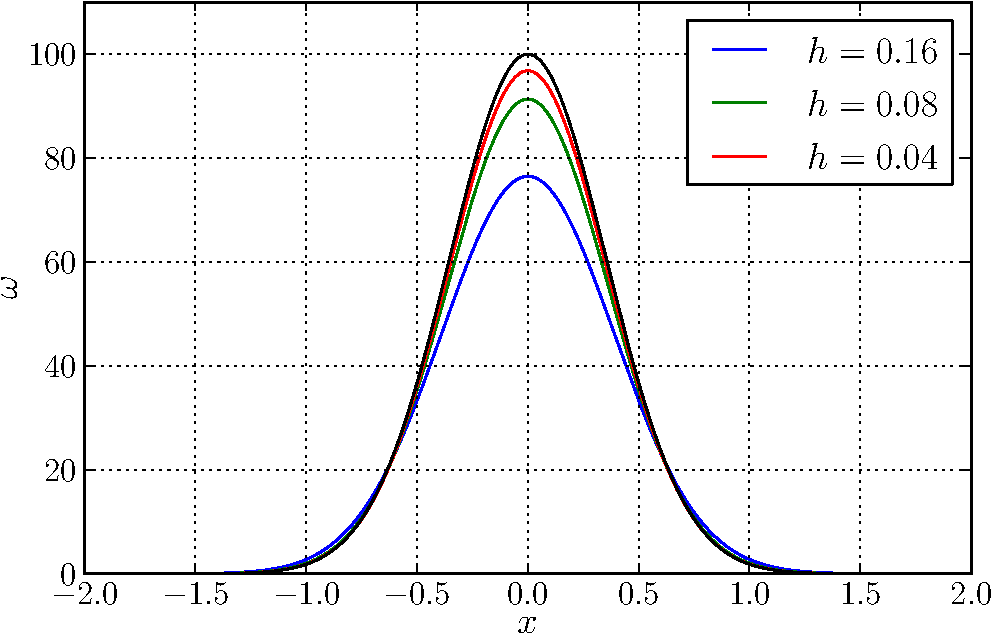
\includegraphics[width=\textwidth]{figures/lagrangian/betterInitialization_h-crop.pdf}
                \caption{Convergence of $h$ with $\lambda = 1.0$}
                \label{fig:convergenceOfBlobsH}
        \end{subfigure}%
        ~ %add desired spacing between images, e. g. ~, \quad, \qquad etc.
          %(or a blank line to force the subfigure onto a new line)
        \begin{subfigure}[b]{0.5\textwidth}
                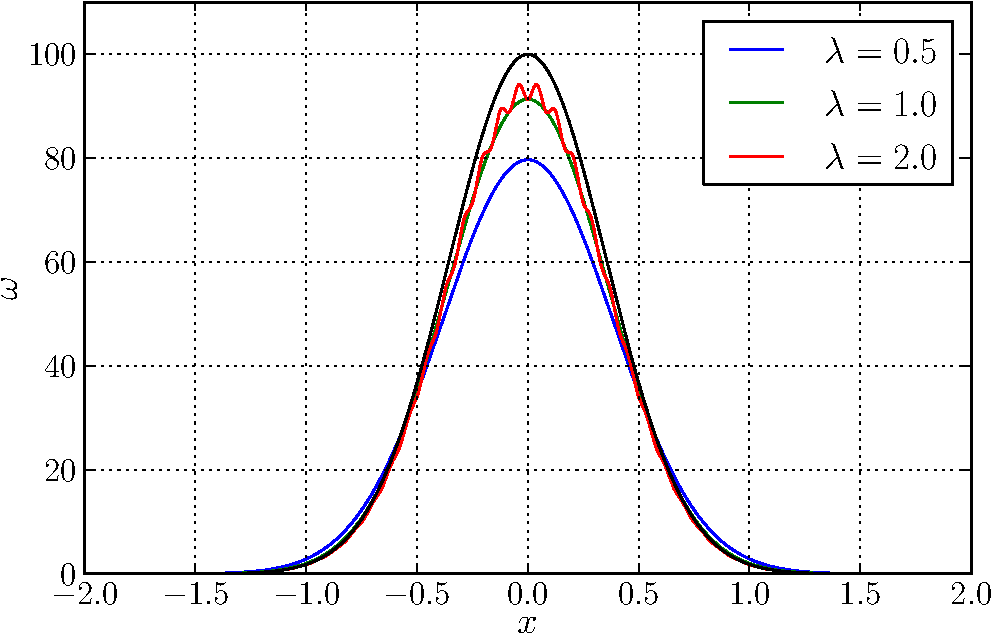
\includegraphics[width=\textwidth]{figures/lagrangian/betterInitialization_overlap_cor-crop.pdf}
                \caption{Convergence of $\lambda$ with $h = 0.08$}
                \label{fig:convergenceOfBlobsOverlap}
        \end{subfigure}
        \caption{Convergence of the spatial discretization $h$ and $\lambda$ of the initial vorticity distribution. Figure depicts the exact vorticity field $\omega$ [---, solid \textbf{black}], and various discretized vorticity distributions.}
        \label{fig:convergenceOfSpatialResolution}
\end{figure}	

Figure \ref{fig:convergenceOfSpatialResolution} shows mollified vorticity field results from modifying the spatial resolution parameters. Figure \ref{fig:convergenceOfBlobsH} shows the convergence of the mollified vorticity field $\omega^h$ to the exact vorticity field $\omega$ by reducing the nominal particle spacing $h$. The overlap ratio is set to $\mathrm{overlap} = 1$, meaning that the blob core-size $\sigma$ is equal to $h$. We see that by reducing blob core size, and simultaneously increasing the number of particles, the mollified vorticity converges to the exact vorticity. 

The second parameter we can adjust is the $\mathrm{overlap}$ of the blobs, as seen in figure \ref{fig:convergenceOfBlobsOverlap}. The blob spacing $h$ is set to $h = 0.08$, and we see that by increasing the overlap ratio $\lambda$, the mollified vorticity approaches the exact vorticity field. However, as shown by Koumoutsakos and Cottett \cite{Cottet2000a}, if the overlap is low, we lose the smooth reconstruction of the vorticity field. This can be seen for $\mathrm{\lambda} = 2.0$. We see that the mollified vorticity field has a fluctuating solution, and will result in non-smooth velocity field.

Thus, to minimize the error in initializing the mollified vorticity $\omega^h$ from the vorticity $\omega$, an overlap ratio of $\lambda = 1.0$, and a small nominal blob spacing $h$ is required. In our hybrid method, this means that at the region where we initialize the vortex blobs (i.e inside the Eulerian domain), we require these conditions to be satisfied. 

\section{Convection in Vortex Particle Method}
\label{sec:covb}

Convection of the vorticity is the first step of evolution of the vorticity from viscous splitting algorithm, from section \ref{subsec:vsa}. The convection of the vorticity is described by the first order hyperbolic equation, equation \ref{eq:convectionEulerian}. The convection equation \ref{eq:convectionEulerian}, is solved by the following system of ordinary differential equations,
	\begin{subequations}
	\begin{align}
	\frac{\mathrm{d}\mathbf{x}_p}{\mathrm{d}t} &= \mathbf{u}\left(\mathbf{x}_p\right),\\
	\frac{\mathrm{d}\alpha_p}{\mathrm{d}t} &= 0,
	\end{align}
	\label{eq:convectionODE}
	\end{subequations}
where the change in position of vortex blob $\mathbf{x}_p$ is due to the induction velocity $\mathbf{u}\left(\mathbf{x}_p\right)$ acting on it, and the strengths of the particles $\alpha_p$ is conserved.

The Biot-Savart Law, equation \ref{eq:mollifiedVelocityField}, is used to determine the induced velocities acting on each particle, resulting in an $N$-body problem. The calculation of the $N$-body problem is optimized by parallelizing the calculations in GPU hardware. The calculation is further optimized by using a fast summation method, the \printAcron{Fast Multipole Method}{FMM}, reducing the problem from $\mathcal{O}(N^2)$ to $\mathcal{O}(N)$ (in the ideal case).

The time integration of equation \ref{eq:convectionODE} is performed using a $4^{\mathrm{th}}$ order explicit Runge-Kutta method. The higher-order time integration ensures an accurate convection of the vortex blobs, resulting in minimum dissipation. However, the downside to employing a multi-stage method is that we require multiple evaluation of the induced velocity $\mathbf{u}\left(\mathbf{x}_p\right)$, when stepping from a given time $t_n$ to the next time $t_{n+1}$.

After several steps of the convection of the vortex blobs, the overlap ratio $\lambda$ will no longer be satisfied due to strains in the fluid, as described by Koumoutsakos and Chorin \cite{Cottet2000a}. In section \ref{subsubsec:convergenceInterpolation}, we determined that to have an accurate reconstruction of the vorticity field, the vortex blobs must satisfy the overlap ratio $\lambda$ at all times $t$. This introduced the need for a remeshing (or a regridding) scheme that can reconstruct the vortex blobs distribution to the original overlap ratio $\lambda$.

\subsection{Remeshing scheme: Treating lagrangian grid distortion}
\label{subsec:remeshing}

The distortion of the Lagrangian grid is due to the clustering and dispersion of the vortex blobs. This clustering and dispersing effect of the blobs is due to the high strains in the flow. Figure \ref{fig:distortion} depicts the distortion of the Lagrangian grid after 100 convection steps. The final distribution shows gaps in vortex blob distribution and will result in an inaccurate representation of the vorticity field. 

	\begin{figure}[!h]
	\centering
	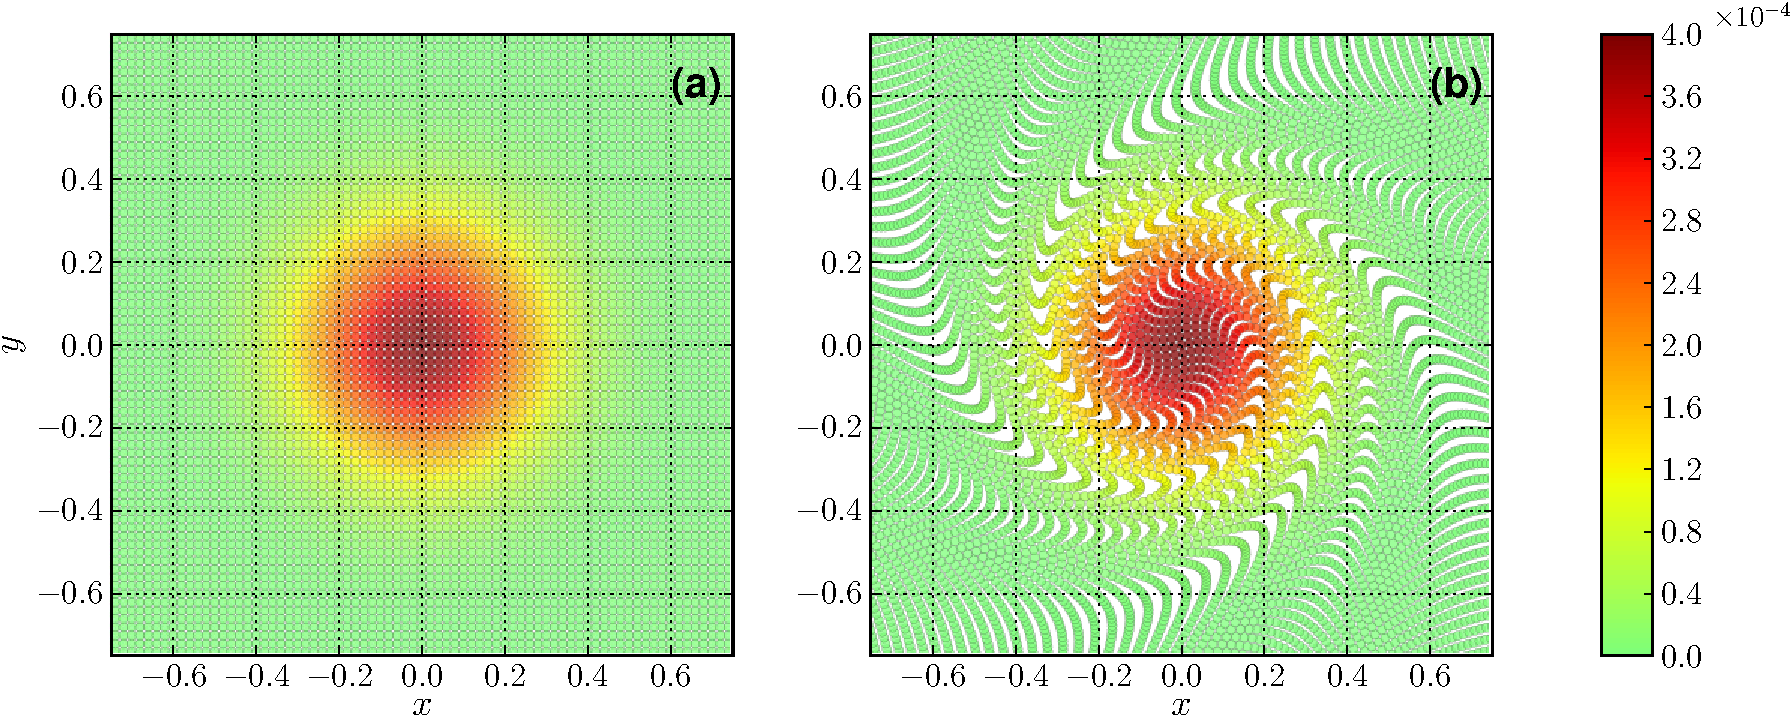
\includegraphics[width=0.9\textwidth]{figures/lagrangian/distortion-crop.pdf}
    \caption{Lagrangian distortion of the vortex blobs after 100 time steps. The initial vorticity field is $\omega\left(\mathbf{x},0\right) = \exp\left(-12\left|\mathbf{x}\right|\right)$ with $\Delta t = 0.1$, $\sigma=0.02$, and $\mathrm{overlap} = 1.0$. Figure depicts $\textbf{(a)}$ the initial distribution of the vortex blobs, and $\textbf{(b)}$ the final distribution of the vortex blobs after 100 time steps.}
    \label{fig:distortion}
	\end{figure}

	\begin{figure}[!b]
	\centering
	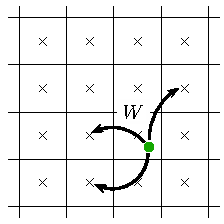
\includegraphics[width=0.4\textwidth]{figures/lagrangian/interpolationGrid.pdf}
	\caption{Remeshing of a single vortex blob [{\color{plotGreen}{$\bullet$}}, green dot] onto a uniform grid defined by the $\left(3\times3\right)$ 2-D stencil.}
	\label{fig:interpolationGrid}
	\end{figure}

A remeshing (or regridding) of this field is therefore required to retain proper distribution. It is done by interpolating the strengths of the vortex blobs from the distorted Lagrangian grid $\hat{\mathbf{x}}$ onto a uniform grid $\mathbf{x}$. The strengths of the blobs of the new uniform grid $\alpha_p$ is determined by,
	\begin{equation}
	\alpha_p = \sum_q\tilde{\alpha}_q W \left(\frac{x_p - \tilde{x}_q}{h}\right),
	\label{eq:la_remeshingKernel}
	\end{equation}
where the strengths of the blobs $\tilde{\alpha}_q$ of the distorted Lagrangian grid $\tilde{x}_q$ are transfered to the regular Lagrangian grid $x_p$ using the interpolation kernel $W$. Figure \ref{fig:interpolationGrid} shows an example of the remeshing of one vortex blob of the distorted grid on to the structured uniform grid with a kernel $W$ with a $3\times3$ stencil. During this transfer, we must ensure that the properties of the fluid are conserved. The interpolation kernel is constructed by ensuring that the total circulation, the linear impulse, and the angular impulse of the fluid are conserved. 

For the present work, the widely used $\mathrm{M}'_4$ interpolation kernel, such as by Koumoutsakos and Cottet \cite{Cottet2000a}, Speck \cite{Speck2011a}, and Barba \cite{Barba2004c}. The kernel is continuously differentiable ensuring conservation of total circulation, linear and angular impulse. 

\subsubsection*{$\mathbf{M}^\prime_4$ interpolation kernel}

The $\mathrm{M}^{\prime}_4$ interpolation kernel is an efficient interpolation kernel that has been used to reconstruct a smooth distribution, and was introduced by Monaghan in 1985 \cite{Monaghan1985}. For a 1D problem, the $\mathrm{M}'_4$ interpolation kernel is defined as,
	\begin{equation}
	{\mathrm{M'}_4}\left( {\xi} \right) =
	  \begin{cases}
	   {1 - \frac{{5{\xi ^2}}}{2} + \frac{{3{{\left| \xi  \right|}^3}}}{2}} & {\left| \xi \right|} < 1, \\
	   \frac{1}{2}{\left( {2 - \left| \xi  \right|} \right)^2}\left( {1 - \left| \xi  \right|} \right) & 1 \leqslant {\left| \xi \right|} < 2,\\
	   0 & 2 \leqslant \left| \xi \right|,
	  \end{cases}
	\label{eq:interpKernel}
	\end{equation}
where
	\begin{equation}
	\xi = \frac{x_{\nu} - x_i}{h},
	\label{eq:xiEquation}
	\end{equation}
	
is a non-dimensional parameter, relating the position of the particle $x_{\nu}$ to the position of the $i^{\mathrm{th}}$ interpolation node $x_i$. The $\mathrm{M'}_4$ is a third-order accurate, piecewise smooth, B-spline kernel. The kernel with the $m = 4$, has a 4 support nodes in each dimension. 

	\begin{figure}[!h]
	\centering
	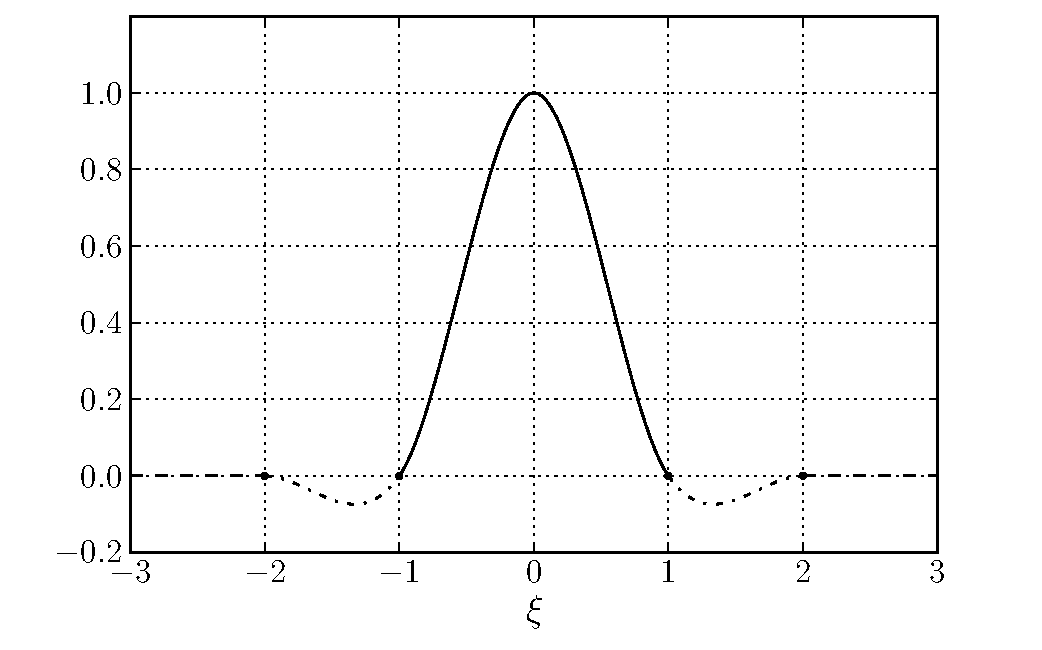
\includegraphics[width=0.6\textwidth]{figures/lagrangian/interpolationKernel.pdf}
	\caption{$M'_4$ interpolation kernel, a third-order, piecewise smooth, B-spline kernel by Monaghan \cite{Monaghan1985}}
	\label{fig:interpolationKernel}
	\end{figure}

Figure \ref{fig:interpolationKernel} shows the distribution of the kernel. For the 2D problem, the 2D interpolation kernel is the tensor product of the 1D interpolation kernel, thus having a $4\time4 = 16$ support nodes. The kernel has a compact support, making it ideal for an efficient $\mathcal{O}(N)$ remeshing.

%Koumoutsakos \cite{Koumoutsakos1997} has investigated the drawback of the employing the remeshing strategy and have shown that there is approximately $4\%$ decay in enstrophy of the flow due to sub-grid dissipation. Note that enstrophy $ \mathcal{E}$, is defined as
%
%% 4 % , give context, what time, how many remshings, say they are negligible for what we do.
%
%	\begin{equation}
%	\mathcal{E} = \frac{1}{2}\int_S \omega^2 dS
%	\end{equation}
%	
%and is directly related to the kinetic energy of the fluid and gives and insight in the energy production and the dissipation of the fluid. Enstrophy is especially useful in turbulence flow investigation as it helps describe the energy cascade of the fluid.		

\section{Diffusion in Vortex Particle Method}
\label{sec:diffusionVM}

Chorin \cite{Chorin1973a}, simulated the viscous flow using the viscous splitting algorithm, described in section \ref{subsec:vsa}. The viscous splitting algorithm segregated the vorticity transport equation, equation \ref{eq:la_vteq}, to the inviscid and the viscous components, equation \ref{eq:convectionEulerian} and equation \ref{eq:vsa2} respectively. 

The flow is convected during the first sub-step, whereas in the second sub-step, we have to deal with the diffusion of the vorticity field, equation \ref{eq:vsa2}. The diffusion problem is solved using the following system of ODEs, 
	\begin{subequations}
	\begin{align}
	\frac{\mathrm{d}\mathbf{x}_p}{\mathrm{d}t} &= 0,\\
	\frac{\mathrm{d}\alpha_p}{\mathrm{d}t} &= \nu\Delta\alpha_p,
	\end{align}
	\label{eq:la_sysODEsDiff}
	\end{subequations}
where the position of the particles $\mathbf{x}_p$ is fixed, whereas the change in strengths of the particles $\alpha_p$ as depended on the kinematic viscous $\nu$. Thus the diffusion of the vortex blobs requires only the modification to the strengths $\alpha_p$ of the particles. 

Chorin in 1973 \cite{Chorin1973a}, initially employed the \indexAcron{Random Walk Method}{RWM}, which generates and disperses vorticity using a pseudo-random number algorithm. However, this method suffered some limitations in accuracy, and since then methods such as \indexAcron{Particle Strength Exchange}{PSE} method \cite{Degond1989a}, and \printAcron{Vortex Redistribution Method}{VRM} \cite{Shankar1996} become a popular choice for treating diffusion of the particles.

The VRM simulates the diffusion of the particles by redistributing fractions of circulations of the vortex blobs to each other, such that diffusion is appropriately modeled. These redistribution fractions $f_{ij}^n$ are determined by solving a linear system of equations, that conserves the moments of the particles (such as the total circulation, linear and angular impulse) and the diffusion of the flow. 

The redistribution fractions $f_{ij}^n$, transfers portion of circulation $\alpha_p$ of the particle $p$ to others within the diffusion radius, defined as,
	\begin{equation}
	h_{\nu} = \sqrt{\nu\Delta t_d}
	\label{eq:la_diffDis}
	\end{equation}
where $h_{\nu}$ is the diffusion distance and is directly related to the kinematic viscosity $\nu$ and the diffusive time step size $\Delta t_d$ of the simulation.

For this work, we investigate two methods that employ this approach. The Wee-Ghoniem Remeshing Scheme \cite{Wee2006a} implemented the VRM into the remeshing process, section \ref{subsec:modifiedRemeshing}. The advantage was that diffusion and remeshing can be performed simultaneously in a single process. However for some flow cases, this approach had undesirable constraint on the diffusion time step size $\Delta t_d$. Therefore, the approach of Tutty \cite{Tutty2010a}, the Tutty Remeshing Scheme, was employed which had a desirable constraint on the diffusion time step size $\Delta t_d$, section \ref{subsubsec:srs}. The scheme was used to perform diffusion at every step of the evolution, which is important for proper coupling of the Eulerian and the Lagrangian method.

%This means that the VRM scheme (and also the PSE) requires a search algorithm to determine the particles that are within the zone of influence. A direct evaluation would require an $\mathcal{O}\left(N^2\right)$ evaluation. However, this can be optimized using a search tree algorithm, speeding up the search to an $\mathcal{O}\left(\log N\right)$.

%Not that the diffusive time-step $\Delta t_d$ is equal to the convective time-step $\Delta t_c$ if the diffusion process is done during every time-step. However, we can easily adjust the diffusion time-step and perform diffusion at a multiple step of the convection. Not diffusing at every step can be helpful as 

%The downside of the this approach, as also for the standard remeshing approach is the global remeshing generates large computation data and scales with the number of particles $N$. Therefore for problems with large number of particles, a tree-structured remeshing would be more feasible strategy \cite{Winckelmans1996}.


\begin{comment}
\subsubsection*{Particle Strength Exchange}
The Particle Strength Exchange method, first proposed by Mas-Gallic in 1989 \cite{Degond1989a}, showed that diffusion can be treated for a particle method with an isotropic, or an anisotropic viscosity by approximating the diffusion operator (a Laplacian) with an integral operator, and discretize the method with particles \cite{Speck2011a}. %The PSE can be seen as circulation correction method, where during the diffusion step of the viscous splitting algorithm, the strengths of the particle are corrected such that it accounts for the diffusion.
 
\subsubsection*{Vortex Redistribution Method}
An alternative method to simulate the diffusion is to use the \printAcron{Vortex Redistribution Method}{VRM} \cite{Shankar1996}. The model simulates diffusion by distributing the fraction of circulation of the vortex blobs to each other satisfying the diffusion. The model is based on conserving the moments of the particles by satisfying a linear system of equations. The circulation of the particle are transfer to the nearby particles that are,
	\begin{equation}
	h_{\nu} = \sqrt{\nu\Delta t_d}
	\end{equation}
where $h_{\nu}$ is the diffusion distance and is directly related to the kinematic viscosity $\nu$ and the diffusive time-step $\Delta t_d$ of the simulation. This means that the VRM scheme (and also the PSE) requires a search algorithm to determine the particles that are within the zone of influence. A direct evaluation would require an $\mathcal{O}\left(N^2\right)$ evaluation. However, this can be optimized using a search tree algorithm, speeding up the search to an $\mathcal{O}\left(\log N\right)$.

%Not that the diffusive time-step $\Delta t_d$ is equal to the convective time-step $\Delta t_c$ if the diffusion process is done during every time-step. However, we can easily adjust the diffusion time-step and perform diffusion at a multiple step of the convection. Not diffusing at every step can be helpful as 

%The downside of the this approach, as also for the standard remeshing approach is the global remeshing generates large computation data and scales with the number of particles $N$. Therefore for problems with large number of particles, a tree-structured remeshing would be more feasible strategy \cite{Winckelmans1996}.

\end{comment}

\subsection{Wee Remeshing Scheme}
\label{subsec:modifiedRemeshing}

Ghoniem and Wee \cite{Wee2006a}, observed the similarities between the VRM and the standard remeshing strategy described in section \ref{subsec:remeshing}. They proposed to combine the remeshing and the diffusion of the vortex blobs together in one single process. The application of this methodology was later investigated by Speck \cite{Speck2011a}. This approach, referred to as the \indexAcron{Wee-Ghoniem Remeshing Scheme}{WRS}, implements the diffusion of the vortex blobs in the interpolation kernel $W$ of equation \ref{eq:la_remeshingKernel}.

The key advantage of the WRS is that, now we are dealing with a uniform grid, and does not require a search algorithm to find the particles in the zone of influence, equation \ref{eq:la_diffDis}. This significantly reduces the computational cost, making this diffusion scheme practical for large scale simulations. 

The modified $\mathrm{M'}_4$ kernel for treating the diffusion is given as,
	\begin{equation}
	{{{\rm{M'}}}_4}\left( {\xi ,c} \right) =
	  \begin{cases}
	   {1 - \frac{{5{\xi ^2}}}{2} + \frac{{3{{\left| \xi  \right|}^3}}}{2} - {c^2}\left( {2 - 9{\xi ^2} + 6{{\left| \xi  \right|}^3}} \right)} & {\left| \xi \right|} < 1, \\
	   \frac{1}{2}{\left( {2 - \left| \xi  \right|} \right)^2}\left( {1 - \left| \xi  \right|} \right) - {c^2}{\left( {2 - \left| \xi  \right|} \right)^2}\left( {1 - 2\left| \xi  \right|} \right) & 1 \leqslant {\left| \xi \right|} < 2,\\
	   0 & 2 \leqslant \left| \xi \right|,
	  \end{cases}
	\label{eq:modInterpKernel}
	\end{equation}
where 
	\begin{equation}
	c^2 = \frac{\nu \Delta t_d}{h^2},
	\label{eq:c2}
	\end{equation}
is a non-dimensional number that corresponds to the transfer weight for the diffusion. The constant $c^2$ is a function of the kinematic viscosity $\nu$, diffusion time step size $\Delta t_d$ and the remeshing grid spacing $h$. This additional term in the interpolation kernel accounts for the diffusion process. When $c \rightarrow 0$, the interpolation kernel simply turns into the standard remeshing kernel, equation \ref{eq:interpKernel}. 

Ghoniem and Wee also investigated the error growth and the stability properties of the interpolation kernel in the Fourier space and have determined that for a stable diffusion and remeshing, the following constraint has to be satisfied,
	\begin{equation}
	\frac{1}{6} \leqslant c^2 \leqslant \frac{1}{2}.
	\label{eq:c2stability}
	\end{equation}

%to minimize the error growth amplification factor and the phase error. With this, we will ensure the stability of the problem and suppress any spurious oscillations and ensure that it is a non-negative interpolation kernel with non-negative redistribution fractions. 
However, we see that this $c^2$ constraint imposes a direct constraint not only on the maximum diffusion time step size $\Delta t_d$, but also imposes a constraint on the minimum step size. This would mean that the diffusion time step size $\Delta t_d$ will be sometimes larger than the convection step $\Delta t_c$,
	\begin{equation}
	\Delta t_d = k_d \cdot \Delta t_c.
	\label{eq:la_dtcts}
	\end{equation}

where $k_d \geqslant 1$ and is an integer. This is a problem for the hybrid method as the Lagrangian method and the Eulerian method are coupled at every step. If the Lagrangian method does not perform diffusion at every step, from the Eulerian method's point of view, it would seem that the Lagrangian vorticity diffuses in a discontinuous fashion. This discontinuous behavior of the Lagrangian method (w.r.t. the Eulerian method), can cause stability issues during the coupling process, and therefore should be avoided.

We could minimize this problem by modifying the $\Delta t_c$ such that it matches the diffusion time step (i.e $\Delta t_c = \Delta t_d$), so that the diffusion is performed at every step. This was a feasible solution for low Reynolds number flows, however for high Reynolds number $Re$ flows, where the convection time step has to be small, we need a scheme that is not constrained by the minimum diffusion time step.

\subsection{Tutty Remeshing Scheme}
\label{subsubsec:srs}

The \printAcron{Tutty Remeshing Scheme}{TRS}, developed by Tutty in 2010 \cite{Tutty2010a}, was based on the VRM of Shankar and Van Dommelen \cite{Shankar1996}. The scheme it possible to remesh and diffuse the vorticity after every convection step. The strengths of the particles after the remeshing and diffusion $\alpha_i^{n+1}$, are given as, 
	\begin{equation}
	\alpha_i^{n+1} = \sum_k \alpha_k^n W_{ki}^n, 
	\end{equation}
where $W_{ki}^n$ is the fraction of circulation transferred from vortex blob $k$ (old) to the new vortex blob $i$ (new), figure \ref{fig:interpolationGrid}. Tutty \cite{Tutty2010a}, explained that the fractions $W_{ki}^n$ are calculated by imposing a conservation of vorticity, center of vorticity, linear, and angular momentum of the vortex blobs, given as,
	\begin{subequations}
	\begin{align}
	\sum_k W_{ki}^n &= 1, \\
	\sum_k W_{ki}^n(x_i - x_k) = \sum_k W_{ki}^n(y_i - y_k) &= 0, \\
	\sum_k W_{ki}^n(x_i - x_k)^2 = \sum_k W_{ki}^n(y_i - y_k)^2 &= 2h_{\nu}^2, \\
	\sum_k W_{ki}^n(x_i - x_k)(y_i - y_k) &= 0,	
	\end{align}
	\label{eq:la_VRMredistributions}
	\end{subequations}
where $h_{\nu}$ is the characteristic diffusion distance associated to the time $\Delta t_d$, 
	\begin{equation}
	h_{\nu} = \sqrt{\Delta t_d \cdot \nu}.
	\end{equation}	

	\begin{figure}[!b]
	\centering
	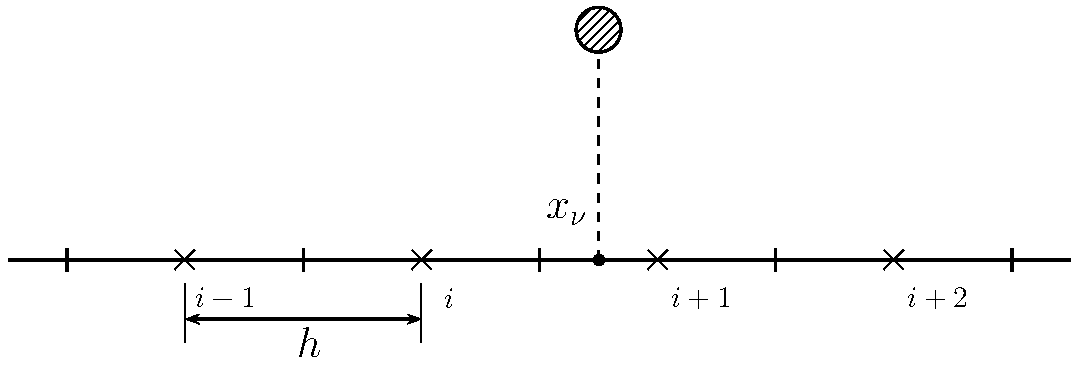
\includegraphics[width=0.7\textwidth]{figures/lagrangian/simpleRedistribution.pdf}
	\caption{1D \printAcron{Tutty Remeshing Scheme}{TRS}, diffusing the vortex blobs at $x_i \leqslant x_{\nu} \leqslant x_{i+1}$, onto the four stencil points $k=i-1,\dots,i+2$, with a grid spacing $h$.}
	\label{fig:simpleRedistribution}
	\end{figure}
	
Similar to the the TRS, described in section \ref{subsec:modifiedRemeshing}, the TRS transfers the strengths to known set of new nodes rather than the neighboring nodes (removing the requirement for a search algorithm). Figure \ref{fig:simpleRedistribution} shows the 1D redistribution of the vortex blob $x_i \leqslant x_{\nu} \leqslant x_{n+1}$ to the stencil nodes $x_k$, where $k=i-1,\cdots,i+2$. The solution to the redistribution is given by the following equations,
	\begin{subequations}
	\begin{align}
	f_{i-1} &= \frac{1}{2}\left(1-f_i-\Delta\right)\\
	f_i &= 1 - 2\left(\frac{h_{\nu}}{h}\right)^2 - \Delta^2\\
	f_{i+1} &= \frac{1}{2}\left(1-f_i+\Delta\right)\\
	f_{i+2} &= 0
	\end{align}
	\end{subequations}
and 	
	\begin{subequations}
	\begin{align}
	g_{i-1} &= 0\\
	g_{i} &= \frac{1}{2}\left(1-g_{i+1}-\Delta_1\right)\\
	g_{i+1} &= 1 - 2\left(\frac{h_{\nu}}{h}\right)^2 - \Delta_1^2\\
	g_{i+2} &= \frac{1}{2}\left(1-g_{i+1}+\Delta_1\right)
	\end{align}
	\end{subequations}
where $\Delta$ is defined as,
	\begin{equation}
	\Delta = \frac{x_{\nu}-x_i}{h},
	\end{equation}
as depicted in figure \ref{fig:simpleRedistribution}. Note that $\xi_1 = \xi - 1$. The total redistribution fractions $F_k$, are the linear combinations of the functions $f_k$ and $g_k$,
	\begin{equation}
	F_k = \left(1-\Delta\right)\cdot f_k + \Delta\cdot g_k, \quad k = i-1,\dots,i+2,
	\end{equation}

For the 2D, the redistribution fractions are simple tensors product of the $x$ and $y$ 1D redistribution fractions,
	\begin{equation}
	W_{kl} = F_k G_l, \quad k = i-1,\cdots,i+2, \quad \l = j-1,\dots,j+2,
	\end{equation}
with a 16 point stencil when $\xi=1/2$.

The stability of the redistribution requires a positive redistribution fraction, $W_{kl}^n > 0$, imposing a direct constraint on the diffusive distance,
	\begin{equation}
	\frac{h_{\nu}}{h} < \frac{1}{\sqrt{2}}.
	\end{equation}
as explained by Tutty \cite{Tutty2010a}. A resulting constraint is imposed on the maximum diffusion time step size $\Delta t_d$,
	\begin{equation}
	\Delta t_d < \frac{h^2}{2\nu}.
	\label{eq:TRS_difftimeconstr}
	\end{equation}

Therefore, we observe that this scheme only poses a constraint on the maximum diffusion time step size $\Delta t_d$, enabling us to perform the diffusion at every step of the evolution, equation \ref{eq:la_dtcts}.

When employing the Tutty's scheme, we require diffusion and redistribution to be performed at every step, i.e the diffusion frequency $f_{diff}=1$ and the redistribution frequency $f_{redis}=1$. In addition to the redistribution, a common approach to minimize the number of vortex blobs is to perform a population control. A population control removes particles with strengths $\left|\alpha\right|$ less than pre-defined circulation threshold $\Gamma_{loc}$, and simultaneously ensuring that the total circulation removed is less that the pre-defined global threshold $\Gamma_{glob}$,

\begin{equation}
\sum_i \left|\alpha_i\right| \leqslant \Gamma_{glob},
\end{equation}

where $\alpha_i$ is the strength of the removed particle $i$. Typically, the population control is performed in conjunction with the redistribution, i.e $f_{redis}=f_{pc}=1$.

%In addition to the remeshing process, we also performed a population control to minimized the number of vortex blobs. After the remeshing process, we may acquire vortex blobs that have negligible influence on other particles, due to its small particle strength. Therefore, we can remove these particles by ensuring that the circulation will be conserved. 


%The one-dimension redistribution fractions for $x$-direction is a linear combination of the two basis solution for a conservative redistribution,
%	\begin{equation}
%	F_k = \left(1-\Delta\right)\cdot f_k + \Delta\cdot g_k, \quad k = i-1,\dots,i+2,
%	\end{equation}
%having a four point stencil, as show in figure \ref{fig:simpleRedistribution}.  

%In the above equation, $h_{\nu}$ is the characteristic diffusion distance during the time $\Delta t_d$, 
%We have to note that, $f_k$ and $g_k$ is zero for all the other $k$. 
%	\begin{equation}
%	h_{\nu} = \sqrt{\Delta t_d \cdot \nu}.
%	\end{equation}
		
%The only constraint imposed for a positive redistribution fraction is,
%
%giving us the maximum time step size constraint of,
%	\begin{equation}
%	\Delta t_d < \frac{h^2}{2\nu}.
%	\end{equation}
	
%Therefore, we observe that this scheme only poses a constraint on the maximum diffusion time step size $\Delta t_d$, enabling us to perform the diffusion at every step of the evolution, equation \ref{eq:la_dtcts}.

\section{Boundary conditions for viscous Vortex Particle Method}
\label{sec:boundaryConditions}

For incompressible viscous flows, the solid boundary is the vorticity generator of the flow. So far, we have only dealt with unbounded flow. For bounded flow simulation, we must enforce the boundary condition of the flow. In 2D, the boundary condition for an immersed body, translating at velocity $\mathbf{u}_b(t)$ with an angular velocity $\Omega(t)$ about it's center of mass $\mathbf{x}_b$ is given as,
\begin{equation}
\mathbf{u}(\mathbf{x}_s) = \mathbf{u}_s
\label{eq:la_bcSlip}
\end{equation}
with,
\begin{equation}
\mathbf{u}_s = \mathbf{u}_b + \Omega(t) \times (\mathbf{x}_s - \mathbf{x}_b),
\end{equation}

where $\mathbf{u}_s$ is the velocity at the surface point $\mathbf{x}_s$. However, in the present work, we deal with stationary bodies and so $\mathbf{u}_b = 0$ and $\Omega(t) = 0$. The boundary condition, Equation \ref{eq:la_bcSlip}, is usually expressed as,
\begin{equation}
\mathbf{u} \cdot \hat{\mathbf{s}} =  \mathbf{u}_s \cdot \hat{\mathbf{s}}.
\end{equation}
equating the tangential components $\hat{\mathbf{s}}$, and is referred to as the \emph{no-slip} boundary condition. The paper of Koumoutsakos, Leonard and Pepin \cite{Koumoutsakos1994b} stated that, by satisfying no-slip boundary condition directly satisfies the no-through boundary conditions, as these boundary conditions are linked (\emph{Linked boundary condition}). This was also been stated by Shiels \cite{Shiels1998} and have been further employed by Cooper, Mar and Barba in 2009 \cite{Cooper2009a}.

	\begin{figure}[!h]
	\centering
	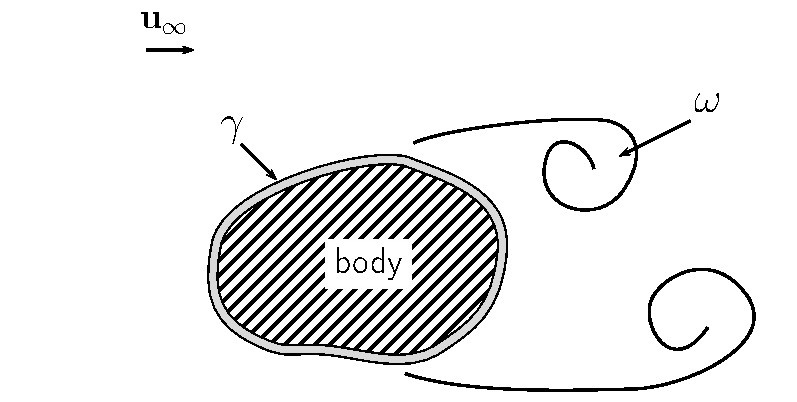
\includegraphics[width=0.6\textwidth]{figures/lagrangian/noSlipVorticityField.pdf}
	\caption{Extended vorticity field separated into vorticity in the fluid and the vortex sheet distribution confined to the body.}
	\label{fig:noSlipVorticityField}
	\end{figure}

Typically in an inviscid flow, the boundary condition is enforced after performing the Helmholtz decomposition of the velocity, equation \ref{eq:helmholtz}. The rotational component $\mathbf{u}_{\omega}$ represents the velocity due to the vorticity in the flow, whereas the potential component $\mathbf{u}_{\phi}$ is used to taken in account of the presence of the body. However, Koumoutsakos, Leonard and Pepin in 1994 \cite{Koumoutsakos1994b}, used an alternate approach for enforcing the boundary condition. Instead of performing the Helmholtz decomposition, they considered an extended vorticity field that is divided into:
\begin{itemize}
\item the vorticity field in the fluid $\omega$,
\item the vortex sheet distribution on the boundary $\gamma$,
\end{itemize}
Figure \ref{fig:noSlipVorticityField} depicts this extended vorticity and the division of the vorticity field to the two sub-categories. The resulting velocity field throughout the domain is given as,
\begin{equation}
\mathbf{u} = \mathbf{u}_{\omega} + \mathbf{u}_{\gamma} + \mathbf{u}_{\infty}
\label{eq:la_noslipbcsimple}
\end{equation}
where $\mathbf{u}_{\omega}$ is velocity field induced by the vorticity in the flow, $\mathbf{u}_{\gamma}$ is the velocity field induced by the vortex sheet and $\mathbf{u}_{\infty}$ is the free-stream velocity.

The vortex sheet distribution $\gamma$ on the boundary is defined by the boundary integral equations, which will be used to enforce the boundary condition.

% Using the Helmholtz decomposition, we can have decompose the velocity field in to the rotational and the irrotational components, equation \ref{eq:helmholtz}. We can use the potential component to prescribe the boundary conditions at the solid wall boundary,
%	\begin{equation}
%	\mathbf{u}_{\phi} = \nabla\Phi.
%	\end{equation}

%The incompressibility constraint results in a Laplace's equation for the potential field and a unique solution is %obtained by enforcing the wall boundary conditions,
%	\begin{equation}
%	\mathbf{u}_b\cdot\mathbf{\hat{n}} = \left(\mathbf{u}_{\omega} + \nabla\Phi\right) \cdot \mathbf{\hat{n}},
%	\label{eq:potentialBC}
%	\end{equation}

%enforcing the no-through flow at the solid boundary wall, moving at $\mathbf{u}_b$, where $\mathbf{\hat{n}}$ is the normal vector of the solid boundary. The approach for determine the solution to the Laplace's equation is by Green's function formulation. This approach required a singularity distribution over the body resulting in the appropriate boundary condition. Doublets and/or source panels are used to attain the required potential such that equation \ref{eq:potentialBC} is satisfied.

%\subsubsection{Linked boundary conditions}

%However Koumoutsakos, Leonard and Pepin in 1994 \cite{Koumoutsakos1994b}, suggested to use vortex sheets to enforce the boundary conditions. This alternate approach of enforcing the solid boundary condition is by not to decompose the velocity field into potential and rotational but to consider the solid boundary as an extension of the vorticity field through vortex sheets $\gamma$, figure \ref{fig:noSlipVorticityField}. Due to the non-zero tangential velocity at the surface, a sudden discontinuity in the velocity field can be considered as vortex sheet. So to enforce the boundary conditions of the solid wall, we must satisfy the no slip velocity at the boundary,
%	\begin{equation}
%	\mathbf{u}\cdot\mathbf{\hat{s}} = \mathbf{u}_b\cdot\mathbf{\hat{s}}.
%	\end{equation}

%Koumoutsakos \cite{Koumoutsakos1993b}, relied only on the vortex sheets to enforce the no-slip velocity. Koumoutsakos, Leonard and Pepin's paper in 1994 \cite{Koumoutsakos1994b} stated that, by satisfying no-slip boundary condition, it directly satisfies the no-through boundary conditions, as these boundary conditions are linked. This was also been stated by Shiels \cite{Shiels1998} and have been further employed by Cooper, Mar and Barba in 2009 \cite{Cooper2009a}. So enforcing the no-slip boundary condition directly satisfies the no-through constraint at the surface.


\subsection{Boundary integral equations}

The Lagrangian method that we are using for the hybrid scheme, is modified according to Stock \cite{Stock2010a}. The Lagrangian method under-resolved the vorticity field in the near-wall region. Furthermore, the vorticity of the fluid is segregated between the vortex blob domain and the vortex sheet domain, as seen in figure \ref{fig:extendedVorticityField}. The figure shows that, very near the wall the vorticity of the fluid is represented by the vortex sheet. In other words, the vortex sheet is an extension to the vorticity represented by the vortex blobs. %The extended velocity field (of the extended vorticity field) is summarized as,
%	\begin{equation}
%	\mathbf{u} = \mathbf{u}_{\omega} + \mathbf{u}_{\gamma} + \mathbf{u}_{\infty}
%	\end{equation}
%where the $\mathbf{u}_{\gamma}$ denotes the velocity field induced by the vortex sheet. 

Enforcing the no-slip boundary conditions, equation \ref{eq:la_noslipbcsimple}, we have that,
	\begin{equation}
	\left(\mathbf{u}_{\mathrm{ext}} + \mathbf{u}_{\gamma}\right)\cdot\mathbf{\hat{s}} = \mathbf{u}_s \cdot \mathbf{\hat{s}}
	\label{eq:kinematicBCofVSOutside}
	\end{equation}
where $\mathbf{u}_{\mathrm{ext}} = \mathbf{u}_{\omega} + \mathbf{u}_{\infty}$ is the velocity field induced from the vortex blob domain (i.e external to vortex sheet domain). The equation states that the tangential component of the total velocity acting on the body should be equal to the tangential velocity of the body. So the induced velocity of the vortex sheet is given as,
	\begin{equation}
	\left(\mathbf{u}_{\mathrm{ext}} - \mathbf{u}_s\right) \cdot \mathbf{\hat{s}} = \mathbf{u}_{\gamma}\cdot\mathbf{\hat{s}}.
	\label{eq:kinematicBCofVS}
	\end{equation}

	\begin{figure}[t]
	\centering
	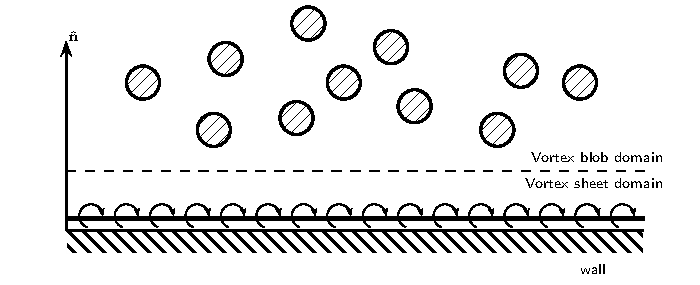
\includegraphics[width=0.8\textwidth]{figures/lagrangian/extendedVorticityField.pdf}
	\caption{Extended vorticity field: Vortex sheet being an extension to the vorticity field (resolved by the vortex blobs), capable of capturing the body bounded vorticity distribution.}
	\label{fig:extendedVorticityField}
	\end{figure}	

Koumoutsakos \cite{Koumoutsakos1993b}, expressed the relation of the vortex sheet strengths to the no-slip boundary condition at the surface of the body (inside the body) through the Fredholm integral equation of the second kind,
	\begin{equation}
	-\frac{\gamma\left(s\right)}{2} + \frac{1}{2\pi}\oint\frac{\partial}{\partial n}\left[\log\left|\mathbf{x}\left(s\right)-\mathbf{x}\left(s'\right)\right|\right]\gamma\left(s'\right)ds'= \mathbf{u}_{\mathrm{slip}}\cdot\mathbf{\hat{s}}.
	\label{eq:fredholmIntegral2ndKind}
	\end{equation}

where $\gamma(s)$ is the strength of the vortex sheet, and $\mathbf{u}_{\mathrm{slip}} = (\mathbf{u}_{\mathrm{ext}}-\mathbf{u}_{b})$, is the slip velocity that needs to be canceled. The \indexAcron{left hand side}{lhs} of the equation states that at the point $\mathbf{x}_s$, the velocity discontinuity is due to the vortex sheet of that point and integral of all the other vortex sheets on the body. However, equation \ref{eq:fredholmIntegral2ndKind} is singular and accepts non-unique solution. 

An additional constraint is obtained from Kelvin's circulation theorem stating that the circulation must be conserved at all times. This imposed a direct constraint on the total circulation of the vortex sheet, defined as,
	\begin{equation}
	\Gamma_{\gamma} = \oint\limits_S\gamma\left(s\right)\ d s.
	\label{eq:circulationConstraintonPanels}
	\end{equation}

where $\Gamma_{\gamma}$ is the integral of the vortex sheet strengths $\gamma$. The total circulation of the vortex sheet $\Gamma_{\gamma}$ is determined during the hybrid coupling of the Lagrangian method to the Eulerian method, see section \ref{subsubsec:cc}.



\begin{comment}
 As the body is in the domain of the vortex sheet, the circulation of the body is represented by the vortex sheet,
	\begin{equation}
	\Gamma_{\mathrm{body}} = \Gamma_{\gamma_{\mathrm{body}}}.
	\label{eq:circulationBody}
	\end{equation}

The circulation of the body is due to the motion of the body traveling at $\mathbf{u}_b$. One can consider the body as filled with uniform vorticity due to the rotation of the body. Therefore the circulation of a moving body can calculated simply integrating the ``vorticity'' inside the body,
	\begin{equation}
	\Gamma_b = \iint\limits_{body} \nabla \times \mathbf{u}_b \ d A.
	\end{equation}	

Furthermore, as we are using the Lagrangian method according to Stock \cite{Stock2010a}, the boundary layer of the body is not resolved with the vortex blobs, as explained in figure \ref{fig:extendedVorticityField}. Therefore, the vortex sheet has to carry this neglected circulation of the boundary layer, and the circulation of the fluid is given as,
	\begin{equation}
	\Gamma_{\mathrm{fluid}} = \Gamma_{\gamma_{\mathrm{BL}}} + \Gamma_{\omega},
	\label{eq:circulationFluid}
	\end{equation}
where $\Gamma_{\gamma_{\mathrm{BL}}}$ is the circulation of the boundary layer region represented by the vortex sheet, and $\Gamma_{\omega}$ is the total circulation captured by the vortex blobs. Combining equation \ref{eq:circulationBody} and \ref{eq:circulationFluid} into equation \ref{eq:circulationNet}, we derive the net circulation of the Lagrangian domain,
	\begin{equation}
	\Gamma = \Gamma_{\gamma_{\mathrm{body}}} + \Gamma_{\gamma_{\omega}} + \Gamma_{\omega} = 0,
	\end{equation}
where the total circulation represented by the vortex sheet is given as,
	\begin{equation}
	\Gamma_{\gamma} = \Gamma_{\gamma_{\mathrm{body}}} + \Gamma_{\gamma_{\mathrm{BL}}}.
	\end{equation}

Thus, the constraint imposed on the net circulation of the vortex sheets is given as,
	\begin{equation}
	\Gamma_{\gamma} = - \Gamma_{\omega}.
	\end{equation}	
ensuring that the total circulation of the fluid is zero. The total circulation of the vortex sheet is calculated by integrating the vortex sheet,
	\begin{equation}
	\Gamma_{\gamma} = \oint\limits_S\gamma\left(s\right)\ d s.
	\label{eq:circulationConstraintonPanelsss}
	\end{equation}	

So we have to solve for the vortex sheet satisfying both the equation \ref{eq:fredholmIntegral2ndKind} and the equation \ref{eq:circulationConstraintonPanelss}, which can be done using a panel method.

%Now, in a pure lagrangian, we must transfer the vorticity generated from the body to the fluid. This is typically done by diffusing the vorticity of the vortex on the fluid, however in our hybrid coupling method, we can use the eulerian domain to introduce the vorticity into the fluid. The eulerian domain acts as the near-wall solver \cite{Daeninck2006}, and the strengths of the particles is interpolated from the eulerian domain, section \ref{}.\todo{CiTe Hybrid sectin}
\end{comment}

\subsection{Discretization of integral equations using vortex panels}

The panel method approach, exposed by Katz and Plotkin \cite{Katz2001a}, is used to solve the set of equations, equation \ref{eq:fredholmIntegral2ndKind} and equation \ref{eq:circulationConstraintonPanels}. Katz and Plotkins have shown several types of panel distributions with various orders of accuracy; from $0^{\mathrm{th}}$ order point vortex or up to $2^{\mathrm{nd}}$ order linear vortex panel. For this work, we have used a constant-strength vortex distribution that discretizes the vortex sheet into straight segments, classified as \indexAcron{Constant-Strength Vortex Panel}{CSVP}.


Equation \ref{eq:fredholmIntegral2ndKind} is solved by discretizing the body surface into $M$ vortex panels, giving us a system of $M$ equation to determine the $M$ unknowns of the strength of the vortex panels.

%This is the panel method, which has been extensively exposed by Katz and Plotkin 


%Panel methods are constructed by discretizing the integral equation \ref{eq:fredholmIntegral2ndKind}, and setting up a system of $M$ equations to solve the $M$ unknowns of the vortex panel,
%	\begin{equation}
%	\underbrace{\begin{pmatrix}
%	-\frac{1}{2} & a_{12} & \cdots & a_{1M}\\ 
%	a_{21} & -\frac{1}{2} & \cdots & a_{2M}\\
%	\vdots & \vdots & \ddots & \vdots\\ 
%	a_{M1} & a_{M2} & \cdots & -\frac{1}{2}
%	\end{pmatrix}}_{\mathbf{A}_{MM}} \underbrace{\begin{pmatrix}
%	\gamma_{1}\\ \gamma_{2}\\
%	\vdots\\
%	\gamma_M\\
%	\end{pmatrix}}_{\vec{\gamma}} = \underbrace{\begin{pmatrix}
%	\mathrm{RHS}_1\\ 
%	\mathrm{RHS}_2\\ 
%	\vdots\\
%	\mathrm{RHS}_M
%	\end{pmatrix}}_{\overrightarrow{\mathrm{RHS}}},
%	\label{eq:vortexSheetSystemofEquations}
%	\end{equation}
%where $A_{MM}$ contains the coefficients of the tangential induced velocity of vortex panels $\vec{\gamma}$ acting on each other. The $\overrightarrow{\mathrm{RHS}}$ is given as,
%	\begin{equation}
%	\mathrm{RHS} = \mathbf{u}_{\mathrm{slip}}\cdot\mathbf{\hat{s}},
%	\end{equation}
%and contains the boundary condition to the system of equations. 

The integral equation \ref{eq:fredholmIntegral2ndKind} is discretized and is given in the matrix form as,
\begin{equation}
\mathbf{A} \cdot \vec{\gamma} = {\overrightarrow{\mathrm{RHS}}},
\label{eq:la_panelProblem}
\end{equation}

where $\mathbf{A}$ is an $M{\times}M$ matrix, containing the coefficients $a_{ij}$, the influence of vortex panel $j$ on the vortex panel $i$. $\vec{\gamma}$ is an $M\times1$ vector contains the strengths $\gamma_i$ of the vortex panel $i$ and ${\overrightarrow{\mathrm{RHS}}}$ contains,
\begin{equation}
\mathrm{RHS}_i = \mathbf{u}_{\mathrm{slip}}\cdot\hat{\mathbf{s}}_i.
\end{equation}

The additional constraint \ref{eq:circulationConstraintonPanels}, is similarly discretized and is given as,
	\begin{equation}
	\sum_{i}^{M} \gamma_i\Delta s_i = \Gamma_{\gamma},
	\label{eq:la_circualtionConstr}
	\end{equation}	
where $\Delta s$ is the length of the vortex panel $i$. Combining the equations, we have a system of $M+1$ equations with $M$ unknowns, given in the matrix form as,
	\begin{equation}
	\underbrace{\begin{pmatrix}
	 a_{11} & a_{12} & \cdots & a_{1M}\\ 
	a_{21} &  a_{22} & \cdots & a_{2M}\\
	\vdots & \vdots & \ddots & \vdots\\ 
	a_{M1} & a_{M2} & \cdots &  a_{MM}\\
	\Delta s_1 & \Delta s_2 & \cdots & \Delta s_M
	\end{pmatrix}}_{\mathbf{B}_{\left(M+1\right)M}} \underbrace{\begin{pmatrix}
	\gamma_{1}\\ \gamma_{2}\\
	\vdots\\
	\gamma_M\\
	\end{pmatrix}}_{\vec{\gamma}} = \underbrace{\begin{pmatrix}
	\mathrm{RHS}_1\\ 
	\mathrm{RHS}_2\\ 
	\vdots\\
	\mathrm{RHS}_M\\
	\Gamma_{\gamma}
	\end{pmatrix}}_{\overrightarrow{\mathrm{RHS}}},
	\end{equation}
Since we now have a set of $M+1$ equations with $M$ unknowns, we have to solve the problem either by using a \indexAcron{Least-Square solution method}{LSTSQ}, or by eliminating an equation as used by Katz, or by the spectral decomposition of the kernel in the Fredholm equation \ref{eq:fredholmIntegral2ndKind}, as used by Koumoutsakos \cite{Cottet2000a}. In this work, we opted for the LSTSQ method that the simplest to implement, however Koumoutsakos showed that to remove the singularity associated to the Fredholm equation \ref{eq:fredholmIntegral2ndKind}, the spectral decomposition method should be used. The singularity becomes a problem with large number of panels, or thin panel geometries.

\subsubsection{Constant-Strength Vortex Panel}

The Constant-Strength vortex panel ({\color{darkblue}CSVP}) is based on the flat (straight) discretization of the vortex sheet, where the panels have constant vortex strength. To solve the strengths of the panel problem, we enforce the Dirichlet velocity boundary conditions at the collocation points $x_{cp}$, that is located just below the vortex sheet, shown in figure \ref{fig:vortexPanelDefinition}. The coefficient $a_{ij}$ of the influence matrix $\mathbf{A}$ ,equation \ref{eq:la_panelProblem}, is defined as,
	\begin{equation}
	a_{ij} = \mathbf{\hat{u}}_{ij} \cdot \mathbf{\hat{t}}_i,
	\end{equation}
which represents the tangential influence coefficient of the $j^{\mathrm{th}}$ panel on the $i^{\textrm{th}}$ panel. The influence coefficient is determined by prescribing the strengths of the vortex panels $\hat{\gamma}_i = 1$, resulting in an induced velocity $\mathbf{\hat{u}}_{ij} = \left(\hat{u},\hat{v}\right)_{ij}$ for a unit strength panel.

	\begin{figure}[!h]
        \centering
        \begin{subfigure}[b]{0.5\textwidth}
                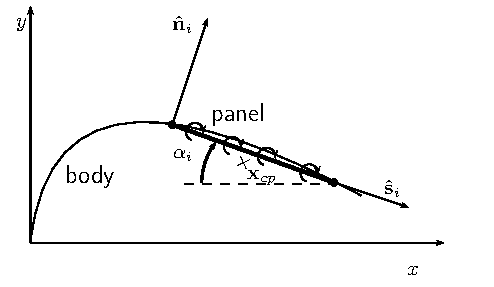
\includegraphics[width=\textwidth]{figures/lagrangian/panelCoordinateDefinition.pdf}
                \caption{Panel discretization of the body in the global cartesian coordinates system $\left(x,y\right)$ with the local panel coordinates system rotated by $\alpha_i$.}
                \label{fig:panelCoordinateDefinition}
        \end{subfigure}%
        ~ %add desired spacing between images, e. g. ~, \quad, \qquad etc.
          %(or a blank line to force the subfigure onto a new line)
        \begin{subfigure}[b]{0.5\textwidth}
                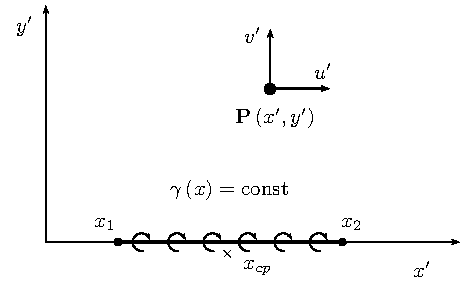
\includegraphics[width=\textwidth]{figures/lagrangian/vortexPanelDefinition.pdf}
                \caption{Constant-Strength Vortex panel in the local panel coordinate system $\left(x',y'\right)$ inducing the velocity $\mathbf{u}'=(u',v')$ on the point $P$.}
                \label{fig:vortexPanelDefinition}
        \end{subfigure}
        \caption{The two coordinate system of the panel method problem. The figure depicts \textbf{(a)} the global panel coordinate system, and \textbf{(b)} the local panel coordinate system, as defined by Katz and Plotkin \cite{Katz2001a}.}
        \label{fig:panelDefinitions}
	\end{figure}	
	
Figure \ref{fig:panelCoordinateDefinition} shows the discretization of the body into panels in the global coordinates system, defined by $(x,y)$, where each panel is rotated by an angle $\alpha_i$ w.r.t to the global coordinate system. Rotating the axis $(x,y)$ by $\alpha_i$, we arrive at the local panel coordinate system $(x',y')$, as shown in figure \ref{fig:vortexPanelDefinition}. Katz and Plotkin \cite{Katz2001a} showed that, the induced velocity of the vortex panels are calculated in the local panel coordinate system, where the induced velocity of the vortex panel $j$ on the collocation point $i$ (in the panel coordinate system) is given as,
	\begin{subequations}
	\begin{align}
	u'_{ij} &= \frac{\gamma_j}{2\pi}\left[\tan^{-1}\frac{y'_i-y'_{j,2}}{x'_i-x'_{j,2}} - \tan^{-1}\frac{y'_i-y'_{j,1}}{x'_i -x'_{j,1}}\right],\\
	v'_{ij} &= -\frac{\gamma_j}{4\pi}\ln\frac{\left(x'_i-x'_{j,1}\right)^2 + \left(y'_i-y'_{j,1}\right)^2}{\left(x'_i-x'_{j,2}\right)^2+\left(y'_i-y'_{j,2}\right)^2}
	\end{align}
	\end{subequations}

where $(x'_1,y'_1)_j$ and $(x'_2,y'_2)_j$ are the coordinates of the panel start and end points in its local panel coordinate system, as shown in figure \ref{fig:vortexPanelDefinition}. The transformation of this vector $(u'_{ij}, v'_{ij})$ to the global coordinates is given as,
	\begin{equation}
	\begin{bmatrix}
	u_{ij}\\
	v_{ij}\\
	\end{bmatrix} = \begin{bmatrix}
	\cos\alpha_j & \sin\alpha_j \\
	-\sin\alpha_j & \cos\alpha_j
	\end{bmatrix} \cdot \begin{bmatrix}
	u'_{ij}\\
	v'_{ij},
	\end{bmatrix}
	\end{equation}

corresponding to a rotation of $\alpha$, as shown in figure \ref{fig:panelCoordinateDefinition}.

If we are dealing with multiple panel bodies (i.e. multiple geometries), as seen in figure \ref{fig:twoPanelBodies}, the panel problem can be solved by constructing a global influence matrix, 
	\begin{equation}
	\underbrace{\begin{pmatrix}
		c_{a_1a_1} & \cdots & c_{a_1a_N} & c_{a_1b_1} &\cdots & c_{a_1b_M}\\
		\vdots & \ddots & \vdots & \vdots &\ddots & \vdots\\
		c_{a_Na_1} & \cdots & c_{a_Na_N} & c_{a_Nb_1} &\cdots & c_{a_Nb_M}\\
		c_{b_1a_1} & \cdots & c_{b_1a_N} & c_{b_1b_1} &\cdots & c_{b_1b_M}\\
		\vdots & \ddots & \vdots & \vdots &\ddots & \vdots\\
		c_{b_Ma_1} & \cdots & c_{b_Ma_N} & c_{b_Mb_1} &\cdots & c_{b_Mb_M}\\
		\Delta s_{a_1} & \cdots & \Delta s_{a_N} & 0 & \cdots & 0\\
		0 & \cdots & 0 & \Delta s_{b_1} & \cdots & \Delta s_{b_M}\\
	\end{pmatrix}
	\begin{pmatrix}
		\gamma_{a_1}\\
		\vdots\\
		\gamma_{a_N}\\
		\gamma_{b_1}\\
		\vdots\\
		\gamma_{b_M}\\
	\end{pmatrix}}_{\begin{pmatrix}
						C_{aa} & C_{ab} \\
						C_{ba} & C_{bb} \\
						\Delta s_a & 0\\
						0 & \Delta s_b \\
					\end{pmatrix} \begin{pmatrix}
								\gamma_{a}\\
								\gamma_{b}\\
							\end{pmatrix}} 
	= 
	\underbrace{\begin{pmatrix}
		\mathrm{RHS}_{a_1}\\
		\vdots\\
		\mathrm{RHS}_{a_N}\\
		\mathrm{RHS}_{b_1}\\
		\vdots\\
		\mathrm{RHS}_{b_M}\\
		\Gamma_{\gamma,a}\\	
	\Gamma_{\gamma,b}
	\end{pmatrix}}_{ 
			\begin{pmatrix}
				\mathrm{RHS}_{a}\\
				\mathrm{RHS}_{b}\\
				\Gamma_{\gamma,a}\\	
				\Gamma_{\gamma,b}
			\end{pmatrix}}
	\end{equation}

where the matrices ($C_{aa}$, $C_{bb}$), are the self-induction matrices of each of the single vortex panel problem. The non-diagonal terms ($C_{ab}$, $C_{ba}$) are the inter-induction matrices containing the panel influence of 
body $b$ on body $a$ and body $a$ on body $b$, respectively. The final two rows of the LHS matrix contain the circulation constraint for each body, defined by equation \ref{eq:la_circualtionConstr}.

	\begin{figure}[t]
	\centering
	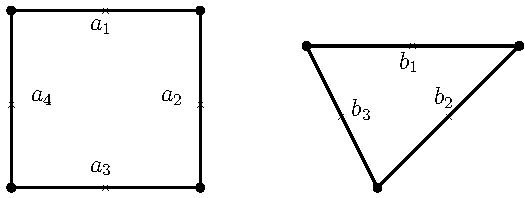
\includegraphics[width=0.6\textwidth]{figures/lagrangian/twoPanelBodies.pdf}
	\caption{Multi-body panel problem: two bodies with different numbers of panels. The figure depicts a square body with 4 panels ($a_1, a_2, a_3, a_4$), and a triangular body with 3 panels ($b_1, b_2, b_3$). }
	\label{fig:twoPanelBodies}
	\end{figure}


%\newpage
%\section{Simulation acceleration techniques}
%\label{sec:sat}
%%
%\subsection{Fast multi-pole Method}
%%
%\subsection{Parallel computation in GPU}


\section{Evolution of the Lagrangian method}

The algorithm of the full Lagrangian method is summarized in this section. The full or complete	Lagrangian method is the coupled vortex blobs and the vortex panels. Note that for our hybrid scheme, the panel does not act as the source of the vorticity in the Lagrangian method (which is done by the Eulerian method), but instead simply enforces the \emph{no-slip} boundary condition for the vortex blobs.
	
	\begin{figure}[!h]
		\centering
		\begin{tikzpicture}
			[node distance=.8cm, start chain=going below,]
			\node[punktchain, join] (solvePanel) {Solve for panels};
		    \node[punktchain, join] (solveVelocity) {Evaluate the total velocity field};
		    \node[punktchain, join] (convect)     {Convect the vortex blobs};
		    \node[punktchain, join] (remesh) 	  {Remesh the Lagrangian field};
		    \node[punktchain, join] (diffuse)     {Diffuse the vortex blobs};		    
		\end{tikzpicture}
		\caption{Flowchart of the Lagrangian method. The flowchart shows coupling between vortex panels and vortex blobs to evolve from $t_n$ to $t_{n+1}$ (without taking into account of the vorticity generation at the boundary).}
		\label{fig:flowchart_lagrangian}
	\end{figure}	
	
The flowchart of one time step of the Lagrangian method is given by figure \ref{fig:flowchart_lagrangian}.The algorithm to the Lagrangian method can be summarized as follows:
	\begin{enumerate}
	\item \textbf{Solve for panels:} Determine the strengths of the vortex panels $\gamma$, such that the no-slip boundary condition at the collocation points of the vortex panels is enforced. When determining the strengths, we also have to ensure that the total circulation of the vortex panels satisfies the conservation of circulation, equation \ref{eq:circulationConstraintonPanels}, which we investigate during the hybrid coupling, section \ref{subsubsec:cc}.
	\item \textbf{Evaluate the total velocity field:} Evaluate the total velocity field $\mathbf{u}$, which is the sum of velocity field induced by the vortex blobs $\mathbf{u}_{\omega}$, the velocity field induced by the vortex panels $\mathbf{u}_{\gamma}$, and the free-stream velocity field $\mathbf{u}_{\infty}$. 
	\item \textbf{Convect the vortex blobs:} Use the velocity field to convect the vortex blobs from $t_n$ to $t_{n+1}$ to the new position.
	\item \textbf{Remesh the Lagrangian field:} Remesh the vortex blobs onto a structured square lattice using the $\mathrm{M}'_4$ interpolation kernel.
	\item \textbf{Diffuse the vortex blobs:} Diffuse the vortex blobs using the $\Delta t_d$ diffusion time step, by modifying the strengths of the vortex blobs according to Wee's WRS or Tutty's TRS method.
	\end{enumerate}

The generation of the vorticity is dealt with in the Eulerian domain, which is explained in chapter \ref{ch:eulerian}. The vorticity is then transfered into the Lagrangian domain using the Hybrid coupling scheme, which was summarized in the introduction, chapter \ref{ch:introduction}, and fully elaborated in chapter \ref{ch:hybrid}.

%
\section{Validation of Lagrangian method}
\label{sec:volm}
In this chapter, we have investigated the Lagrangian component of the Hybrid method. The Lagrangian method is used to just evolve the vorticity field, where as the Eulerian method is used to properly formulate the vorticity generation at the boundary. The resolved boundary solution of the Eulerian method is then transfered onto our Lagrangian method. Therefore, the Lagrangian method that is implemented here does not require the generation of the vorticity from the boundary. 

Thus, during the validation of the Lagrangian method, we focus on two test cases: Potential flow around a cylinder and Lamb-Oseen vortex evolution. The potential flow around a cylinder test case is used to verify and validate the vortex panel solver that is used enforcing the no-through flow for the vortex blobs. The Lamb-Oseen vortex evolution test cases is used to verify and validate the convection method and the diffusion methods implemented for the evolution of the vortex blobs.

Note that to investigate the coupling of the vortex blobs and the vortex panels, we require the proper definition of the vorticity flux from the boundary, requiring the Eulerian method as well. Therefore, the handling of the vorticity flux is investigated in fully coupled method, in chapter \ref{ch:vavohm}.


\subsection{Error analysis of vortex panels}

	\ctable[
	    caption = {Panel study parameters},
	    label   = {tab:panelParams},
	    pos = b,
	]{lll}{}{\FL
	Parameters 				& Value 			& Description \ML
	$R$  					& 1 \si{m} 			& Radius of cylinder\\
	$u_{\infty}$	& 1 \si{m.s^{-1}}	& Free-stream velocity\\
	$N_{\mathrm{panels}}$	& 100				& Number of panels\LL}	

The vortex panels was verified and validated on the test case of the potential flow around a cylinder. To test the 
convergence of the solution of the vortex panels, a comparison was made with the analytical solution for the parameters in table \ref{tab:panelParams}.

An example of the numerical solution is shown in figure \ref{fig:panelCylinder_velocityField}. The figure shows the magnitude of the velocity $\lVert\mathbf{u}\rVert|$, and it shows the velocity field of the potential flow solution, with an infinitely thin boundary layer, stagnating to zero velocity inside the body.

	\begin{figure}[p]
	\centering
	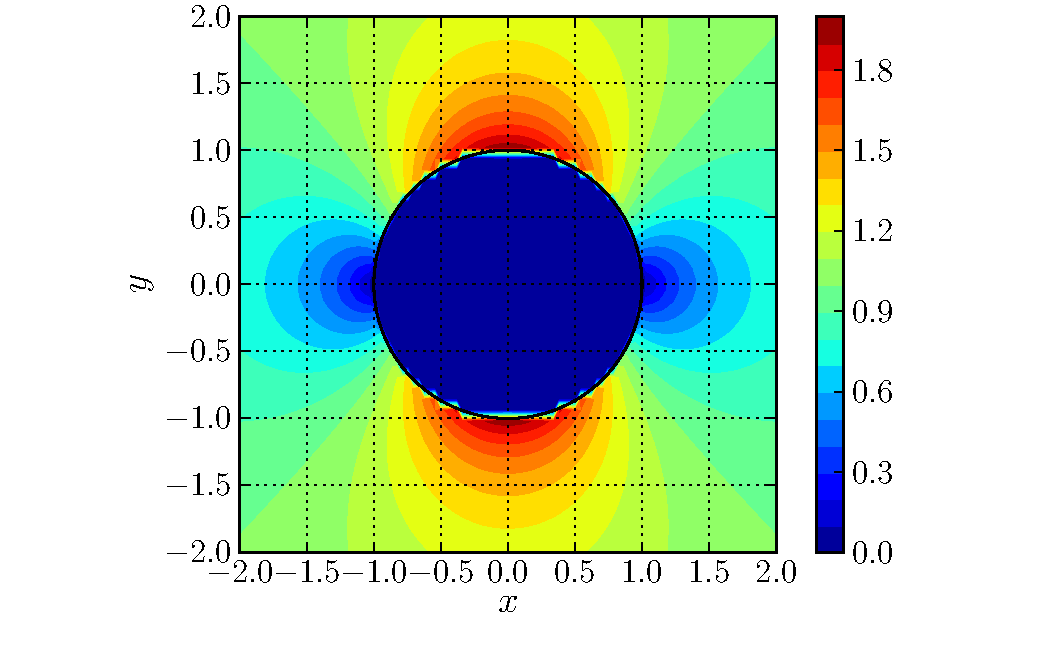
\includegraphics[width=0.7\textwidth]{figures/lagrangian/panelCylinder_velocityField.pdf}
	\caption{Panel method solution: the potential velocity field around a unit cylinder with $R = 1$, $\mathbf{u}_{\infty} = (1, 0)$, and $N_{\mathrm{panels}}=100$. The figure depicts the magnitude of velocity field $\left\Vert\mathbf{u}\right\Vert$, with a zero velocity inside the body.}
	\label{fig:panelCylinder_velocityField}
	\end{figure}

	\begin{figure}[p]
     \centering
     \begin{subfigure}[b]{0.5\textwidth}
             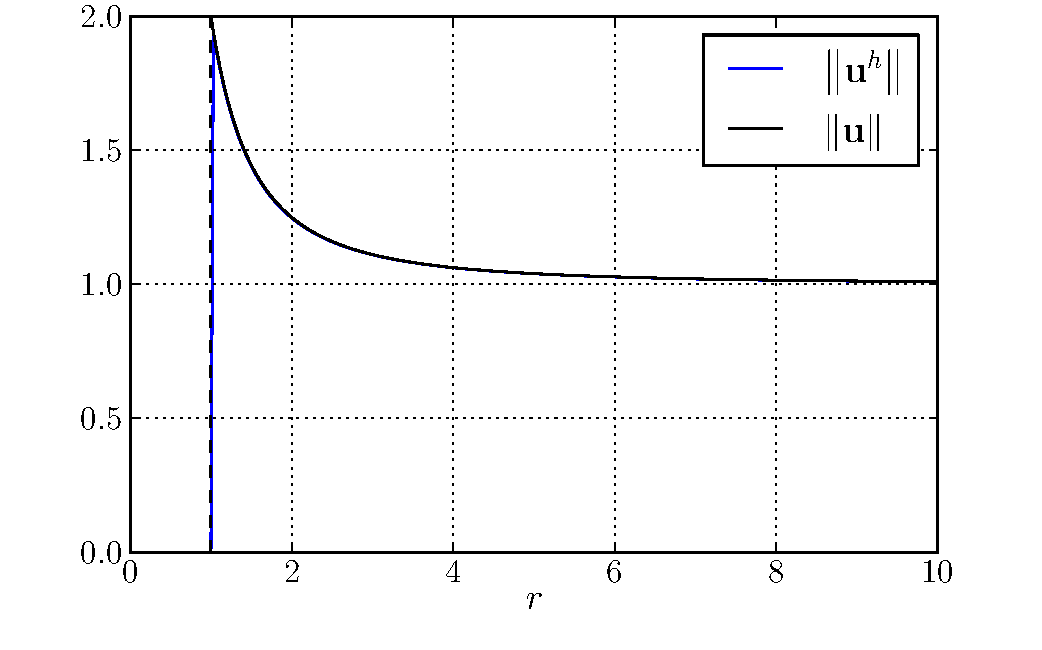
\includegraphics[width=\textwidth]{figures/lagrangian/panelCylinder_versusAnalytical.pdf}
             \caption{Comparison of the velocity field.}
             \label{fig:panelCylinder_versusAnalytical}
     \end{subfigure}%
     ~ %add desired spacing between images, e. g. ~, \quad, \qquad etc.
       %(or a blank line to force the subfigure onto a new line)
     \begin{subfigure}[b]{0.5\textwidth}
             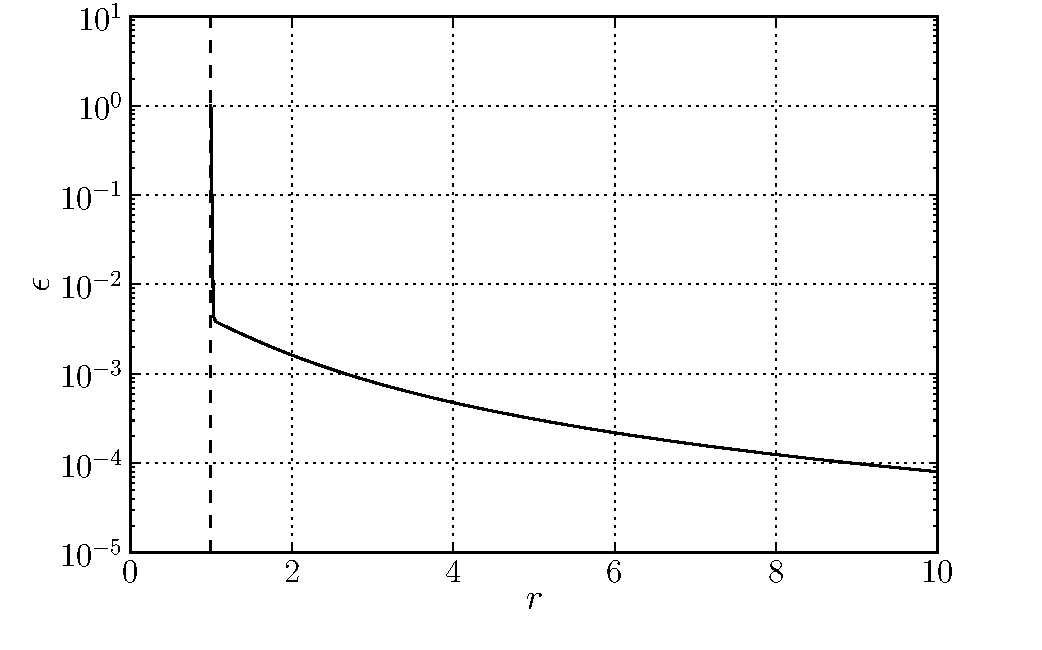
\includegraphics[width=\textwidth]{figures/lagrangian/panelCylinder_error.pdf}
             \caption{Error in the velocity field}
             \label{fig:panelCylinder_error}
     \end{subfigure}
     \caption{Comparison of the velocity field along the $y$-axis, $0\rightarrow10$. Figure \textbf{(a)} shows both the solutions, the numerical $\left\Vert\mathbf{u}^h\right\Vert$ [{\color{plotBlue}{---}}, solid blue] and the analytical solution [---, solid black]. Figure \textbf{(b)} shows the relative error $\epsilon$ in velocity between the solution, given by equation \ref{eq:panelRelativeError}.}
     \label{fig:panelCylinderComparision}
	\end{figure}

	\begin{figure}[p]
	\centering
	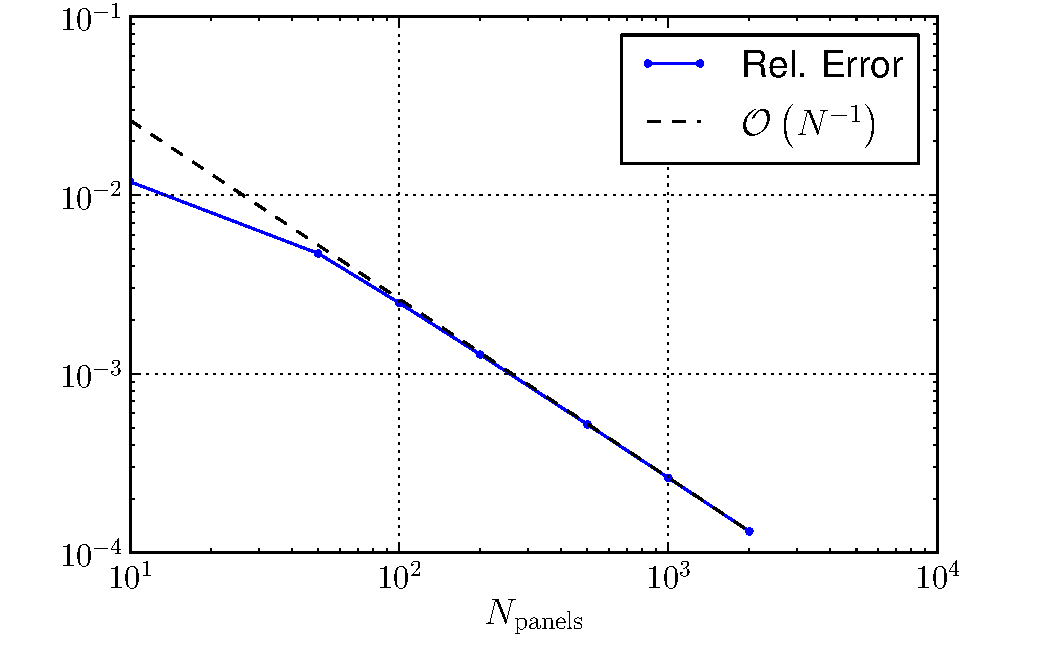
\includegraphics[width=0.5\textwidth]{figures/lagrangian/panelCylinder_convergence_compressed.pdf}
	\caption{Convergence plot of the Constant-Strength Straight Vortex panels. The figures depicts the converges of the relative error $\epsilon$ at an $\mathcal{O}\left(N^{-1}\right)$.}
	\label{fig:panelCylinder_convergence}
	\end{figure}


The jagged velocity field around the surface of the cylinder is simply due to the sampling resolution of the field. For a higher sampling resolution this will vanish. In order to determine the accuracy of the solution, the velocity field of the panel solution was compared with the analytical solution. The analytical velocity field around a cylinder is given in cylindrical coordinate centered in the cylinder as,
	\begin{subequations}
	\begin{align}
	u_r &= u_{\infty}\left(1 - \frac{R^2}{r^2}\right)\cos\theta,\\
	u_{\theta} &= -u_{\infty}\left(1+\frac{R^2}{r^2}\right)\cos\theta,
	\end{align}
	\label{eq:potentialCylinderAnalytical}
	\end{subequations}	
where $u_r$ and $u_{\theta}$ are the radial and the angular velocity respectively for a given free-steam velocity $u_{\infty}$. Equation \ref{eq:potentialCylinderAnalytical} is a function of the distance to the center of the cylinder $r$ and the radius of the cylinder $R$ and is valid for $r\geqslant{R}$

The velocity field of the vortex panel was compared with the analytical solution along the y-axis from $y=0$ to $y=10$. Figure \ref{fig:panelCylinder_versusAnalytical} plots the magnitude of analytical velocity $\left\Vert\mathbf{u}\right\Vert$ and the vortex panel velocity field $\left\Vert\mathbf{u}^h\right\Vert$. Comparing the solutions of the plot we see that the solution of the vortex panels and the analytical potential flow solution matches everywhere except at the surface. This happens because the potential flow solution has a slip velocity (i.e non-zero velocity) at the surface of the body, whereas the vortex panels solves for a no-slip boundary condition at the collocation points of the surface. This explains the sudden drop of the velocity from $\lVert\mathbf{u}\rVert = 2$ to $\lVert\mathbf{u}\rVert = 0$ at the surface.	

Figure \ref{fig:panelCylinder_error} shows the relative error $\epsilon$ between the numerical and the analytical solutions,
	\begin{equation}
	\epsilon = \frac{\left\Vert\mathbf{u}-\mathbf{u}^h\right\Vert}{\left\Vert\mathbf{u}\right\Vert}
	\label{eq:panelRelativeError}
	\end{equation}
	
where $\mathbf{u}$ is the analytical solution and the $\mathbf{u}^h$ is the numerical solution. Ignoring the solution right at the surface ($r=R$), we see that the error between the numerical and the analytical solution reduces from $\epsilon=\num{5e-3}$ to $\epsilon=\num{8e-5}$ as we go from $r=1$ to $r=10$. This behavior of the error tells us that the solution of the constant-strength vortex panels gets more accurate as we go further away from the panels; right next to the panels, we have the largest error.

The convergence analysis of the vortex panels was done by determining the error of the vortex panel velocity field w.r.t to the analytical solution for the number of panels $N = 10$ to $N = 1000$, figure \ref{fig:panelCylinder_convergence}. The error of the velocity field was computed at $(x =0, y=1.5)$, and we see that the error converges at with $\mathcal{O}\left(N\right)$. This validates that the vortex panel that we have used is a $1^{\mathrm{st}}$ order vortex panel.

\subsection{Error analysis of vortex blobs}
\label{subsec:lagrangianLambOseen}
In order to verify and validate the vortex blobs, we simulate the evolution of a Lamb-Oseen vortex. The results of the simulation were used to compare against the analytical ones, which we used to determine the accuracy of our vortex blobs.

The Lamb-Oseen vortex is a solution of the Navier-Stokes equation, corresponding to the viscous evolution of a laminar vortex core on an unbounded domain, first derived by Lamb and Oseen \cite{Tryggeson2007}. The vorticity distribution $\omega$ of the core at a given time is defined as,

	\begin{equation}
	\omega\left(\mathbf{x},\tau\right) = \frac{\Gamma_c}{4\pi\nu(t+\tau)} \exp\left(-\frac{r^2}{4\pi\nu(t+\tau)}\right),
	\label{eq:lo_voeq}
	\end{equation}

and is a function of core strength $\Gamma_c$, the simulation time $t \in [0,\infty[$ and distance from the core center $r$. The constant $\tau$ in the equation \ref{eq:lo_voeq} defines to initial width of the Lamb-Oseen vortex, where if $\tau=0$, we have Dirac delta distribution.

The velocity field, corresponding to equation \ref{eq:lo_voeq}, in cylindrical coordinate is defined as,

	\begin{subequations}
	\begin{align}
	u_{\theta} &= \frac{\Gamma_c}{2\pi r} \left[1-\exp\left(-\frac{r^2}{4\pi\nu(t+\tau)}\right)\right]\\
	u_r &= 0
	\end{align}
	\label{eq:lo_veeq}
	\end{subequations}

where $u_{\theta}$ is the circumferential velocity, and $u_r$, the radial velocity is zero. Figure \ref{fig:lambOseen_distributions} shows the vorticity distribution $\omega$ for various initial time constant $\tau$. We see that for small $\tau$, the distribution approaches a Dirac delta distribution. Therefore, for this investigation we decided on $\tau=4$ ensuring a non-peaky distribution, which was also investigated by Barba \cite{Barba2004c}.  Therefore the literature of Barba \cite{Barba2004c} will serve as the validation data for our Lamb-Oseen investigation.


%	\begin{figure}[!t]
%        \centering
%        \begin{subfigure}[b]{0.5\textwidth}
%                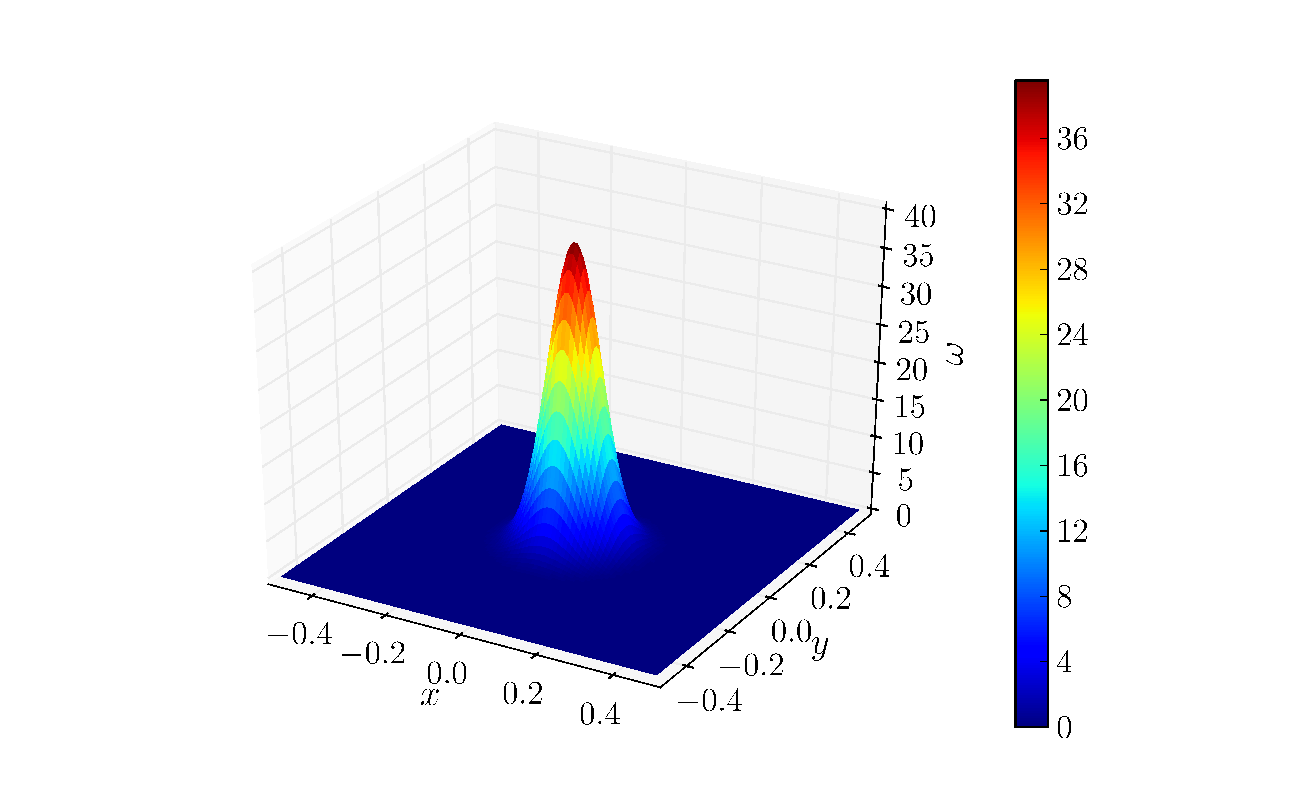
\includegraphics[width=\textwidth]{figures/lagrangian/lambOseen_vorticityDistribution_compressed.pdf}
%                \caption{Vorticity field}
%                \label{fig:lambOseen_vorticityDistribution}
%        \end{subfigure}%
%        ~ %add desired spacing between images, e. g. ~, \quad, \qquad etc.
%          %(or a blank line to force the subfigure onto a new line)
%        \begin{subfigure}[b]{0.5\textwidth}
%                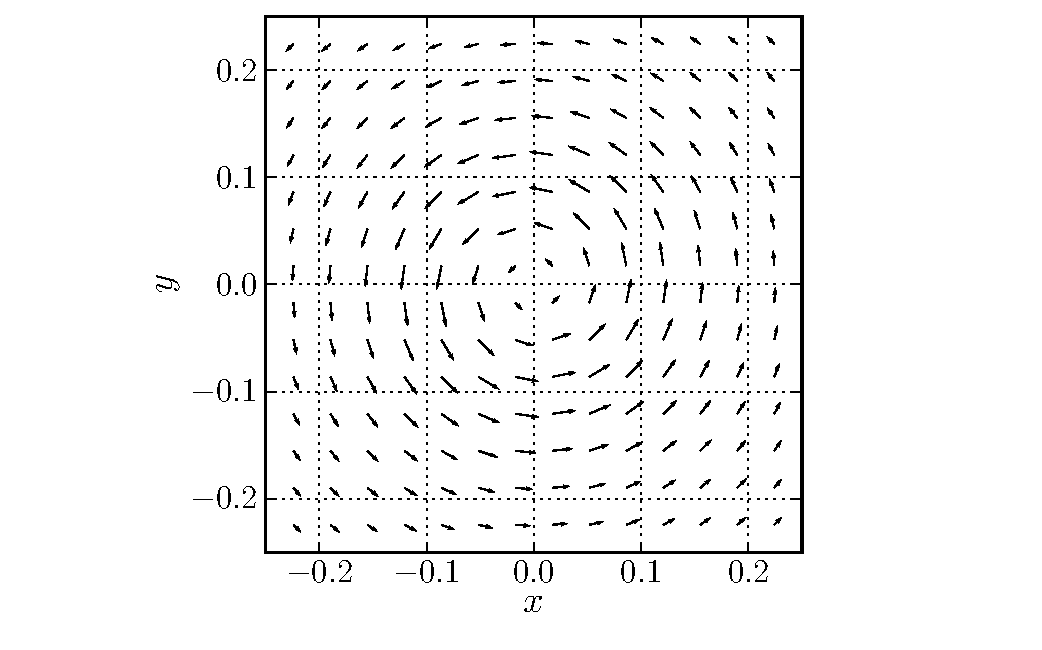
\includegraphics[width=\textwidth]{figures/lagrangian/lambOseen_velocityDistribution_compressed.pdf}
%                \caption{Velocity Field}
%                \label{fig:lambOseen_velocityDistribution}
%        \end{subfigure}
%        
%        
%        \caption{Lamb-Oseen Vortex problem with $\Gamma_c = 1$, $\tau=\num{2e-3}$, and $\nu=\num{5e-4}$. The figure depicts \textbf{(a)} the vorticity distribution, and \textbf{(b)} the velocity distribution.}
%        \label{fig:lambOseen_distributions}
%	\end{figure}

	\begin{figure}[!t]
        \centering
        \begin{subfigure}[b]{0.3\textwidth}
                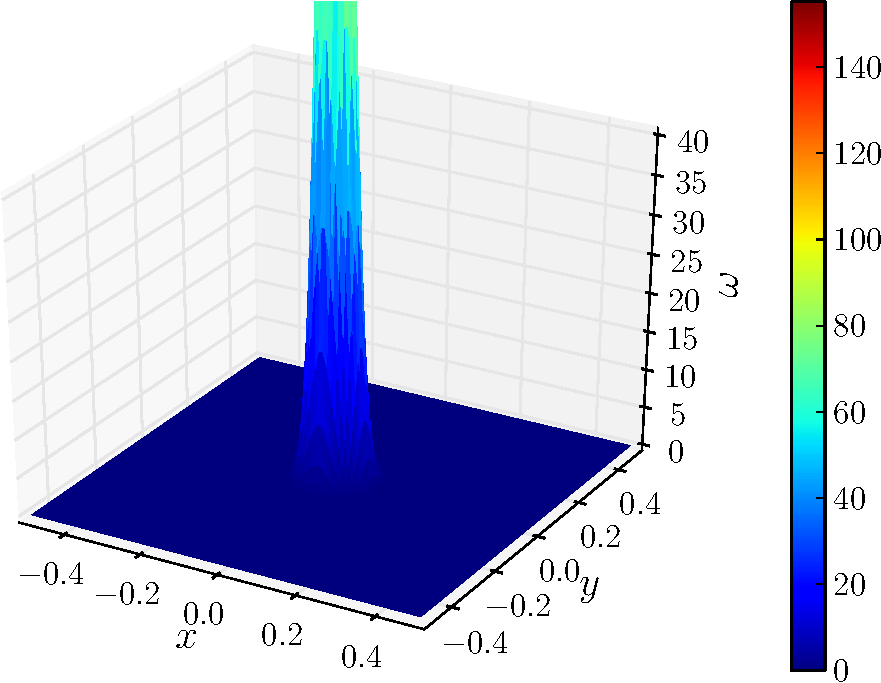
\includegraphics[width=\textwidth]{figures/lagrangian/lambOseen_definition_tau=1-crop.pdf}
                \caption{$\tau = 1$}
                \label{fig:lambOseen_tau1}
        \end{subfigure}%
        ~ %add desired spacing between images, e. g. ~, \quad, \qquad etc.
          %(or a blank line to force the subfigure onto a new line)
        \begin{subfigure}[b]{0.3\textwidth}
                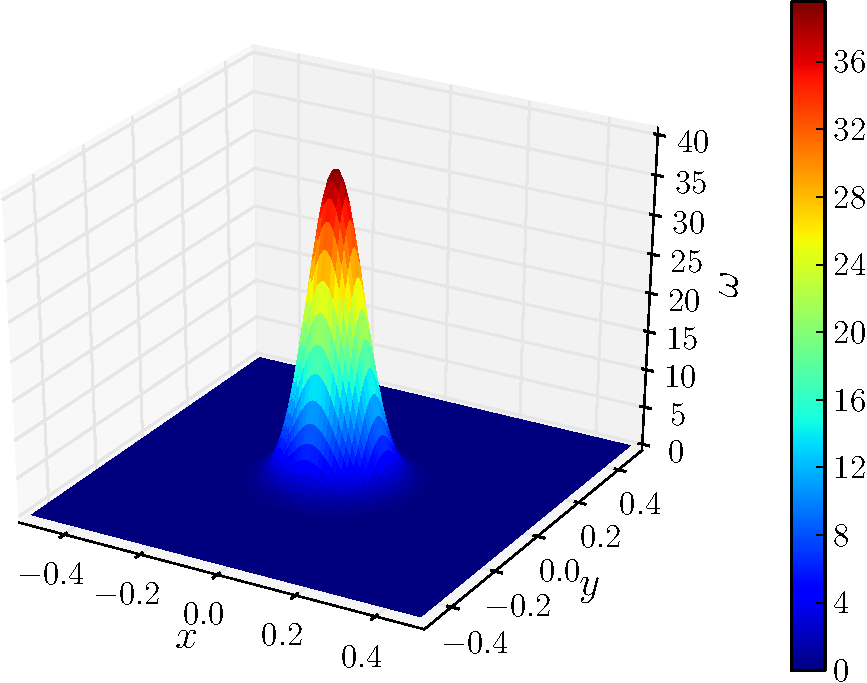
\includegraphics[width=\textwidth]{figures/lagrangian/lambOseen_definition_tau=4-crop.pdf}
                \caption{$\tau = 4$}
                \label{fig:lambOseen_tau4}
        \end{subfigure}
		~
        \begin{subfigure}[b]{0.3\textwidth}
                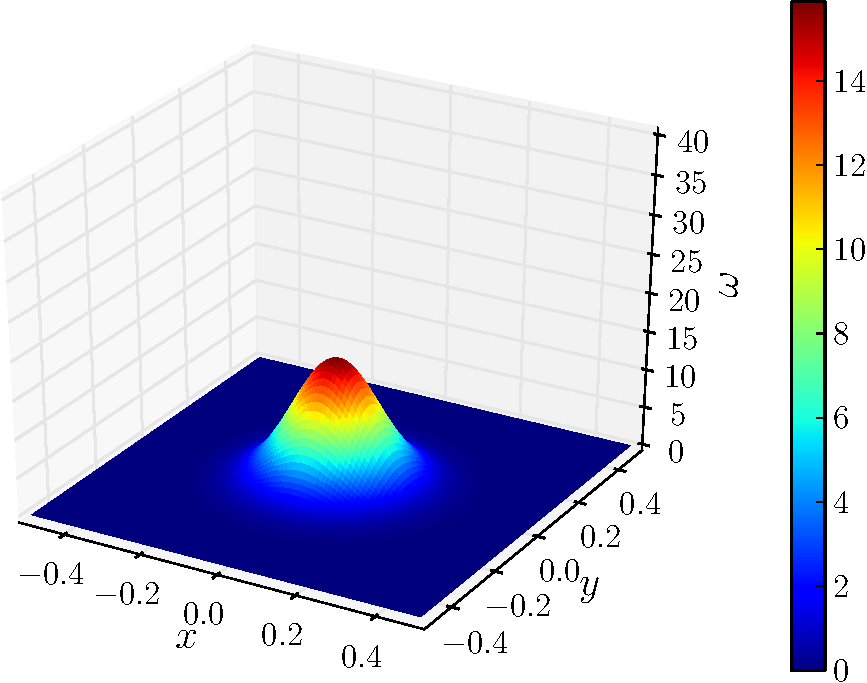
\includegraphics[width=\textwidth]{figures/lagrangian/lambOseen_definition_tau=10-crop.pdf}
                \caption{$\tau = 10$}
                \label{fig:lambOseen_tau10}
        \end{subfigure}        
        
        \caption{The vorticity $\omega$ distribution of the Lamb-Oseen vortex problem with $\Gamma_c = 1$ and $\nu=\num{5e-4}$ in the domain $[-0.5,0.5]\times[-0.5,0.5]$. The figure depicts distribution for various initial time constant $\tau$, determining the peakiness of the distribution.}
        \label{fig:lambOseen_distributions}
	\end{figure}
	
	
	\ctable[
		caption = {Summary of the parameters for the Lamb-Oseen vortex evolution. This table shows also the parameters of Tutty's diffusion method},
		label   = {tab:lambOseenParams},
		pos = !b,]{lcll}{}{\FL
		
		Parameters 					& Value 	& Unit					& Description \ML
		$\Gamma_c$\T               	& 1 &\si{m^2.s^{-1}} 				& Core strength\\
		$\Omega$               		& $\left[-0.5,0.5\right]\times\left[-0.5,0.5\right]$ &\si{m}	& Initial particle domain \\
		$\mathbf{u}_{\infty}$ 		& $0$ &\si{m.s^{-1}} & Free-stream velocity\\
		$\nu$						& $\num{5e-4}$ &\si{kg.s^{-1}.m^{-1}}& Kinematic viscosity\\
		$ \tau$ 		    		& 4		& \si{s}					& Lamb-Oseen time constant\\
		$ t$ 		    	& \numrange{0}{1} &\si{s}			& Simulation time\\		
		$ \Delta t_c = \Delta t_d$ 	& $0.01$ &\si{s}						& Diffusion and convection time step size\\
		$ N_{\mathrm{t-steps}}$ 	& 100 & -						& Number of time integration steps\\		
		$ \sigma$ 					& $0.01$ &\si{m}						& Vortex blob core size\\	        
		$ \lambda$			& $1$	& -							& Overlap ratio\\	        	        
		$ k$						& $2$	& -							& Gaussian kernel width spreading\\
		$ f_{redis}$		& $1$ 	& -							& Redistribution frequency\\	        	        
		$ f_{pc}$		& $1$  & -							& Population control frequency\\	        	        
		$ (\Gamma_{loc},\Gamma_{glob})$ & $(\num{1e-14},\num{1e-14})$ &\si{m^2.s^{-1}} & Population control thresholds\LL}	

The Lagrangian method was applied to the Lamb-Oseen vortex test case with parameters tabulated in table \ref{tab:lambOseenParams}. The vorticity field was discretized over the domain $[x,y]$ - domain $\left[-0.5,0.5\right]\times\left[-0.5,0.5\right]$. This was adequate as the circulation outside this domain was less that the threshold $\Gamma_{loc}\le\num{e-14}$. The spatial discretization was performed according to the standard initialization method of vortex blobs, described in section \ref{subsec:vortexBlobInitialization}.

However as explained in section \ref{subsec:vortexBlobInitialization}, we have to take in account of the Gaussian blurring of the original vorticity field due to the initialization process. This poses a problem when evaluating the error between the numerical and the analytical solution. This problem has also been encountered by Barba \cite{Barba2004c}, when investigating the Lamb-Oseen vortex. The solution to the problem was to apply a ``time-shift correction", to compensate for the Gaussian blurring, solving the problem of this very particular discretization of the Navier-Stokes equation. Therefore, this is a special method and this approach can only be used for the Lamb-Oseen vortex problem.

The ``time-shift correction" is derived by determining the diffusion effect caused by the discretization of the diffusion equation using the Gaussian vortex blobs (with $k=2$). Barba \cite{Barba2004c}, determined that the discretization of the diffusion equation (i.e. the Lamb-Oseen vortex) reconstructs the vorticity field that has been diffused by a time $\sigma^2/2\nu$. So when initializing the particles with a certain strength, we will have to reverse the time by $\sigma^2/2\nu$. Thus, the corrected initial particles strengths $\alpha_i^o$ of vortex blobs from the Lamb-Oseen vorticity field is given as,

	\begin{equation}
	\alpha_i^o = \omega_i^o\cdot h^2 = \left\{ \frac{\Gamma_c}{4\pi\nu\left(t+\tau-\sigma^2/2\nu\right)} \exp\left[-\frac{r_i^2}{4\nu\left(t+\tau-\sigma^2/2\nu\right)}\right] \right\} \cdot h^2.
	\label{eq:lo_pie}
	\end{equation}
	
This method was used to investigate the error evolution of the vortex blob method. The vortex blobs where convected according to the procedures in section \ref{sec:covb}. The diffusion of the vortex blobs was performed using the schemes described in section \ref{sec:diffusionVM}. We investigated the accuracy of the Tutty's scheme (TRS) and Wee-Ghoniem scheme (WRS) in section \ref{subsubsec:comp_wrs_trs}. For the general investigation however, we employed the Tutty's diffusion method. The advantage of this approach is that the we can perform diffusion after every convection step. This makes the method less prone to time integration error and eliminates any discontinuous behavior in the evolution. We will see that when coupling the Lagrangian method and Eulerian method, discontinuity in the problem introduces additional errors.

%	\begin{figure}[p]
%	\centering
%	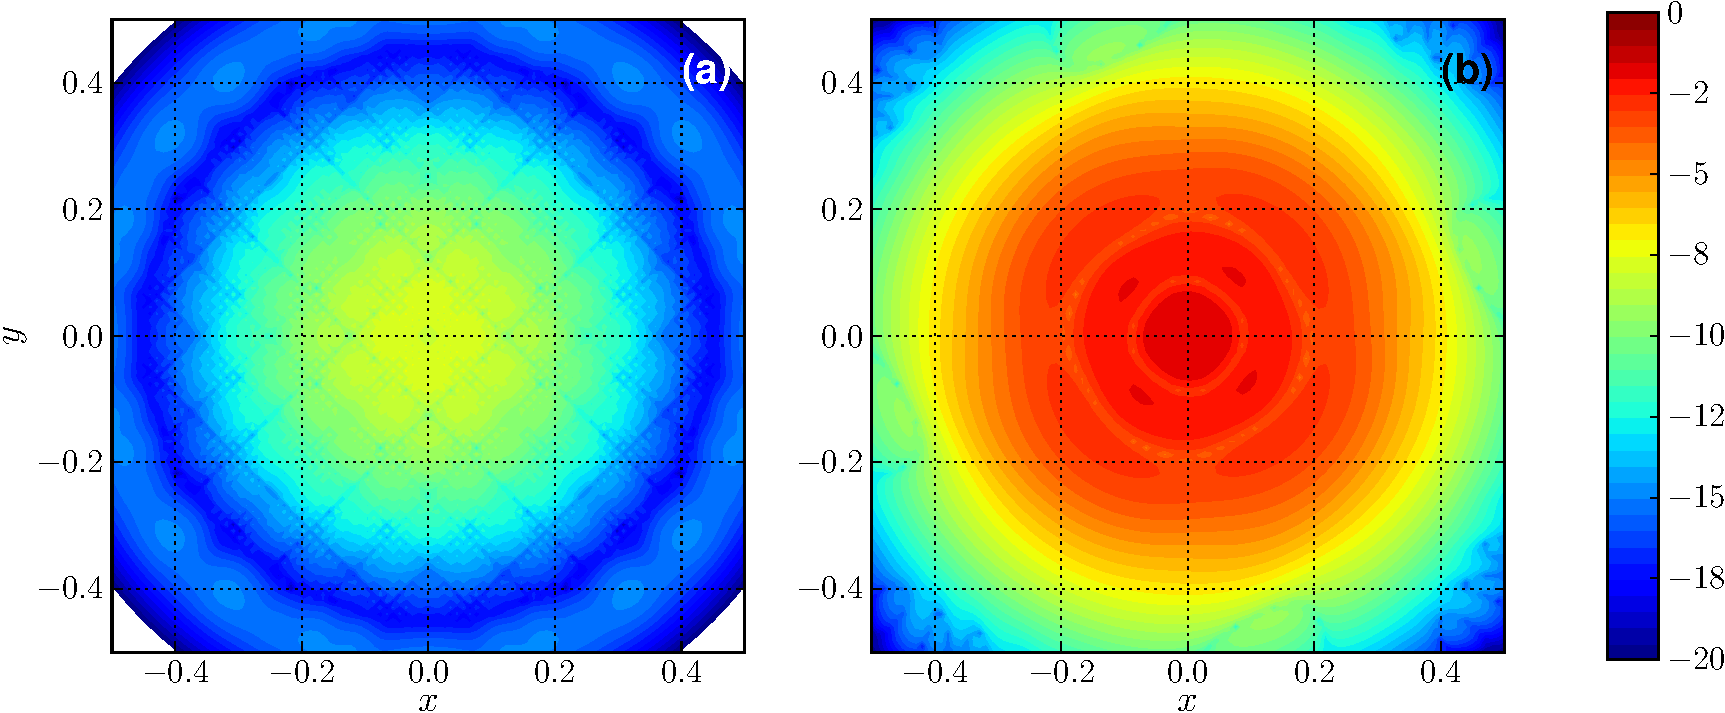
\includegraphics[width=0.99\textwidth]{figures/lagrangian/lambOseen_convection_vorticityErrorContours_compressed-crop.pdf}
%	\caption{Relative error growth of Lamb-Oseen vorticity during the evolution (in logarithmic scale). The figure shows \textbf{(a)}, the initial relative error at $t_0=4$, and \textbf{(b)} the final relative error in vorticity at $t_f=5$.}
%	\label{fig:lambOseen_convection_vorticityErrorContours_compressed}
%	\end{figure}
%	
	


The convection and diffusion was performed according to the time integration parameters tabulated in table \ref{tab:lambOseenParams}. The vortex blobs where convected using a $4^{\mathrm{th}}$-order Runge-Kutta method ($\mathrm{RK4}$) for a high order time integration. After the convection sub-steps, the Lagrangian distortion was treated using the remeshing scheme discussed in section \ref{subsec:remeshing}. Generally, the remeshing is typically done every 10 iterations \cite{Barba2004c}. However, as our diffusion scheme and hybrid method requires structured lattice of vortex blobs for efficient calculations, we will remesh after every step, $f_{\mathrm{redist}}=1$.  


In addition to the evolution of the vortex blobs, we performed a population control to minimized the number of vortex blobs, as described by Barba \cite{Barba2004c}. The \indexAcron{Population Control}{PC} removes vortex blobs that have very small circulation strengths. After the diffusion and remeshing, we will be left with vortex blobs with strengths close to the numerical precision, as they have minimal impact on the accuracy of the vorticity field, we can removed them. When performing population control, we need to ensure that the loss of total circulation is below the acceptable global threshold, $\Gamma_{glob}$. We used $\Gamma_{glob}=\num{e-14}$ as used by Barba \cite{Barba2004c} for the similar investigation. 

	\begin{figure}[!h]
     \centering
     \begin{subfigure}[b]{0.5\textwidth}
             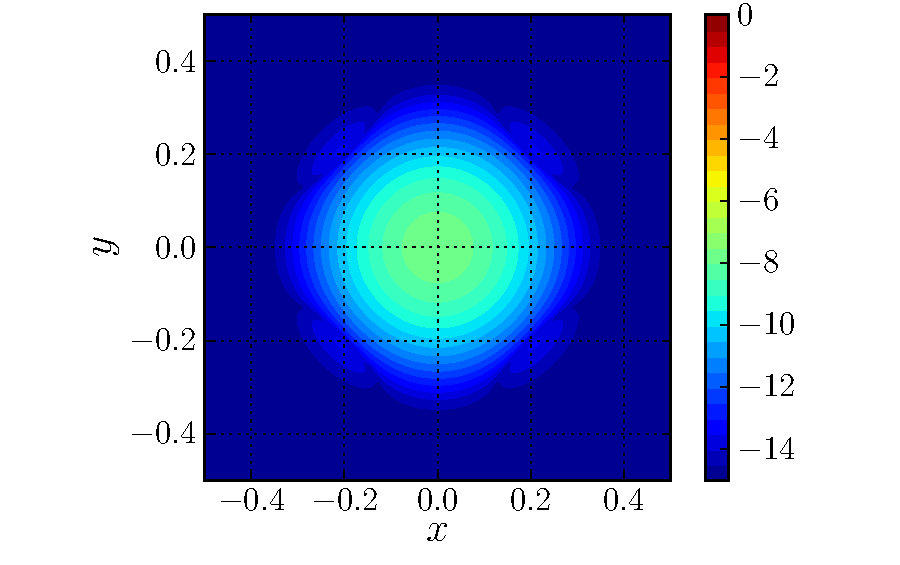
\includegraphics[width=\textwidth]{figures/lagrangian/lambOseen_intialError_wRel.pdf}
             \caption{Vorticity field}
             \label{fig:lambOseen_convection_vorticityErrorContours_initial}
     \end{subfigure}%
     ~ %add desired spacing between images, e. g. ~, \quad, \qquad etc.
       %(or a blank line to force the subfigure onto a new line)
     \begin{subfigure}[b]{0.5\textwidth}
             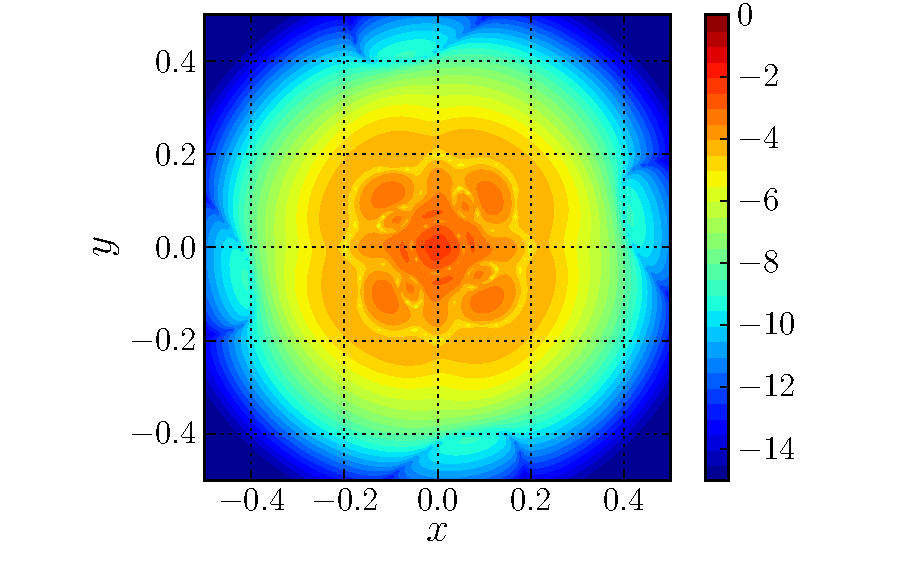
\includegraphics[width=\textwidth]{figures/lagrangian/lambOseen_finalErrorEvolution_wRel.pdf}
             \caption{Velocity Field}
             \label{fig:lambOseen_convection_vorticityErrorContours_final}
     \end{subfigure}
     
     \caption{Relative error growth of Lamb-Oseen vorticity during the evolution (in logarithmic scale) using the parameters tabulated in table \ref{tab:lambOseenParams}. The figure shows \textbf{(a)}, the initial relative error at $t=0$, and \textbf{(b)} the final relative error in vorticity at $t=1$.}
     \label{fig:lambOseen_convection_vorticityErrorContours}
	\end{figure}

To verify whether our Lagrangian scheme is performs according to theory, we evaluated the error evolution of the simulation. Figure \ref{fig:lambOseen_convection_vorticityErrorContours}, shows the initial and the final relative error in vorticity. We see that initially we have a maximum relative error around \num{e-8}, located at the center of the Lamb-Oseen core. After 100 time integration steps from $t=0$ to $t=1$, we see that the maximum relative error in vorticity increases from \num{e-8} to \num{e-2}. The errors of the vorticity are predominantly localized at the center of the core, where we have maximum vorticity, figure \ref{fig:lambOseen_convection_vorticityErrorContours}.

Figure \ref{fig:lambOseen_convection_errorGrowth_compressed}, shows the maximum relative error, equation \ref{eq:maxRelErrorDef}, and the $L^2-\mathrm{norm}$, equation \ref{eq:l2normeq}, error evolution of vorticity and velocity from $t=0$ to $t=1$. Similar investigation was performed by Barba \cite{Barba2004c} and Speck \cite{Speck2011a}. Due to the relation of the vorticity and the velocity, equation \ref{eq:lag_vort}, the error of the vorticity is higher that the error in the velocity. The figure shows both the maximum relative error, and the error in the $L^2-\mathrm{norm}$. The maximum relative error (e.g. for vorticity), is defined as,
	\begin{equation}
	\left\Vert \omega^{\mathrm{exact}} - \omega^{\mathrm{discrete}} \right\Vert_{\infty} = \frac{\max\{\left|\omega^{\mathrm{exact}} - \omega^{\mathrm{discrete}}\right|\}}{\max\{\left|\omega^{\mathrm{exact}}\right|\}},
	\label{eq:maxRelErrorDef}
	\end{equation}
where $\omega^{\mathrm{exact}}$ is the analytical vorticity field, equation	\ref{eq:lo_voeq}, and $\omega^{\mathrm{discrete}}$ is the numerical vorticity field from the vortex blobs. The error in the $L^2-\mathrm{norm}$ of the vorticity is calculated as 

	\begin{equation}
	\left\Vert \omega^{\mathrm{exact}} - \omega^{\mathrm{discrete}} \right\Vert_2 = \left(\sum_{i}^{N}\left| \omega^{\mathrm{exact}} - \omega^{\mathrm{discrete}} \right|^2 \cdot h^2\right)^{\frac{1}{2}},
	\label{eq:l2normeq}
	\end{equation}

and the error in velocity is calculated using the same principle. Investigating the figure, we see that after the first iteration, there is a sudden increase in the error, but as time progresses the error growth reduces. From literature, we see that this trend has also been observed by Barba \cite{Barba2004c} and Speck \cite{Speck2011a}. For comparison, we used similar parameters, and we observe that the sudden jump in error is similar to the literature.

	\begin{figure}[!h]
	\centering
	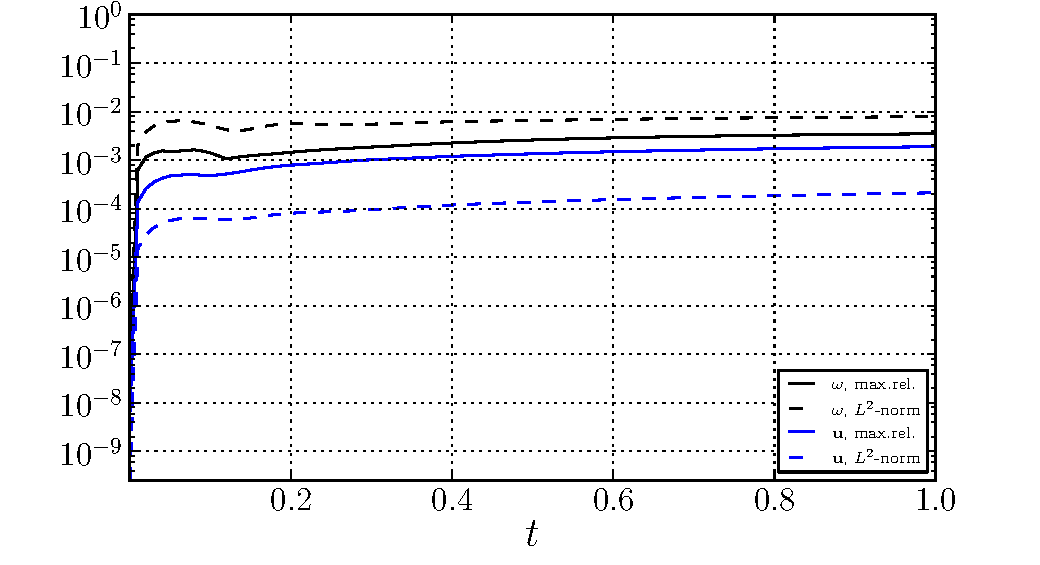
\includegraphics[width=0.6\textwidth]{figures/lagrangian/lambOseen_errorEvolution_TRS_dt0p01.pdf}
	\caption{Relative error growth of Lamb-Oseen vortex during the evolution from $t=0$ to $t=1$ using the parameters in table \ref{tab:lambOseenParams}. This figure depicts the error in vorticity: maximum relative error [ ---, solid black], and the error in $L^2-\mathrm{norm}$ [ - -, dashed black]; and error in velocity: maximum relative error [ {\color{plotBlue}{---}}, solid blue], and error in $L^2-\mathrm{norm}$ [ {\color{plotBlue}{- -}}, dashed blue].}
	\label{fig:lambOseen_convection_errorGrowth_compressed}
	\end{figure}

	
\subsubsection{Comparison of diffusion schemes: WRS vs. TRS}
\label{subsubsec:comp_wrs_trs}
To observe how both the diffusion schemes compare, we ran the same test case with both diffusion schemes. From the simulation, we were able to observe that Tutty's diffusion scheme (TRS), produced less error than Wee's approach (WRS). 

Figure \ref{fig:lambOseen_diffusionMethod_comparison} shows the evolution of maximum relative error in vorticity, equation \ref{eq:maxRelErrorDef} for both diffusion schemes. Figure \ref{fig:lambOseen_errorEvolution_WRSvsTRS_dt0p01} shows the evolution of error for convective time step size $\Delta t_c = 0.01$. The diffusion scheme TRS enables us to perform diffusion in conjunction with the convection, $\Delta t_d = \Delta t_c = 0.01$. This was possible due to the favorable constraint on the diffusion time step, equation \ref{eq:TRS_difftimeconstr}.

The Wee's diffusion scheme WRS, however is constraint by equation \ref{eq:c2stability} and equation \ref{eq:la_dtcts}. Therefore the diffusion time step $\Delta t_d$ for the given convective time step $\Delta t_c = 0.01$ is $\Delta t_d = k_d \cdot \Delta t_c = 0.07$, where the diffusion frequency $k_d=7$. We observe from the figure that performing diffusion at every other instant creates an oscillatory behavior. This behavior is not ideal when coupling with the Eulerian method as the oscillatory diffusion of the VPM will add additional error in coupling.

\begin{figure}[!h]
  \centering
  \begin{subfigure}[b]{0.5\textwidth}
          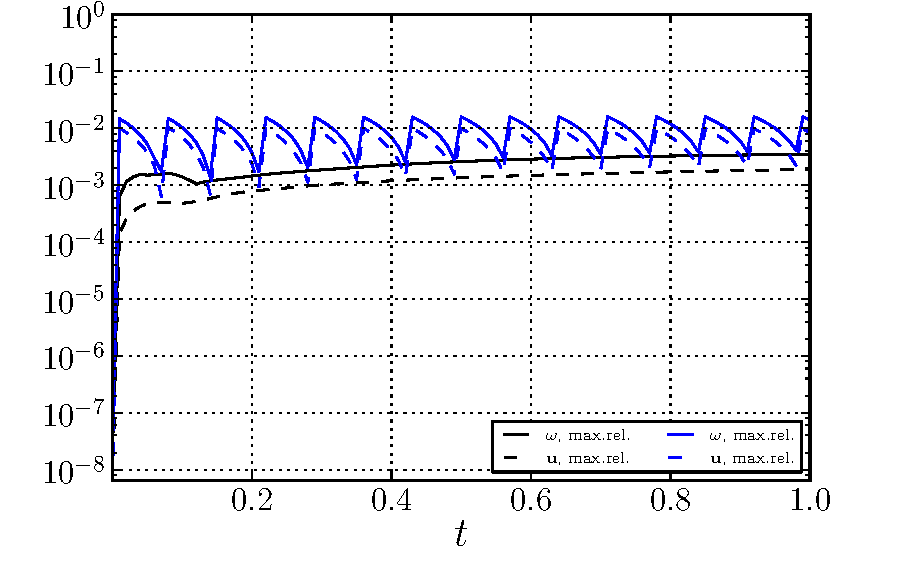
\includegraphics[width=\textwidth]{figures/lagrangian/lambOseen_errorEvolution_WRSvsTRS_dt0p01.pdf}
          \caption{$\Delta t_c = 0.01$}
          \label{fig:lambOseen_errorEvolution_WRSvsTRS_dt0p01}
  \end{subfigure}%
  ~ %add desired spacing between images, e. g. ~, \quad, \qquad etc.
    %(or a blank line to force the subfigure onto a new line)
  \begin{subfigure}[b]{0.5\textwidth}
          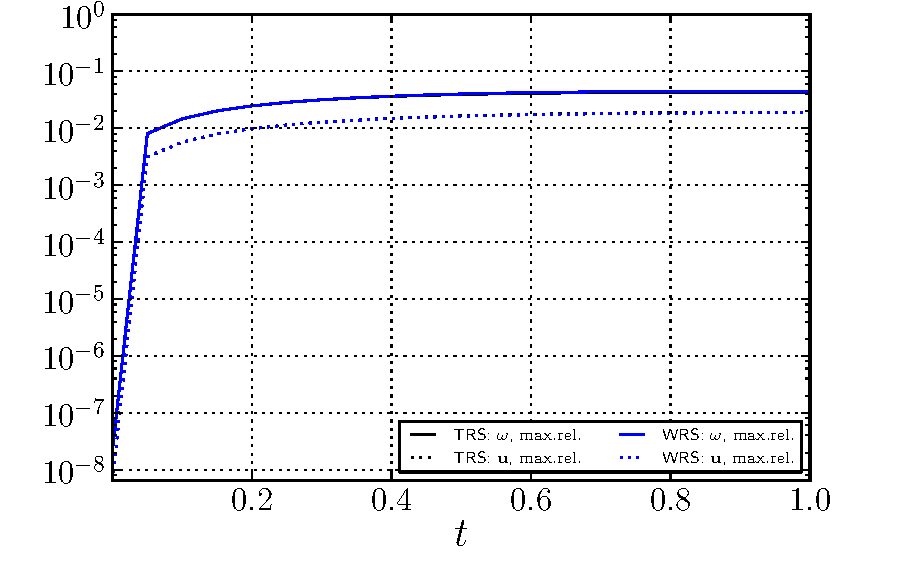
\includegraphics[width=\textwidth]{figures/lagrangian/lambOseen_errorEvolution_WRSvsTRS_dt0p05.pdf}
          \caption{$\Delta t_c = 0.05$}
          \label{fig:lambOseen_errorEvolution_WRSvsTRS_dt0p05}
  \end{subfigure}
  
  \caption{Comparison of Tutty's scheme TRS, and Wee-Ghoniem scheme WRS for treating diffusion, depicting the evolution of maximum relative error in vorticity, equation \ref{eq:maxRelErrorDef} from $t=0$ to $t=1$. The figure \textbf{(a)} shows TRS performing diffusion at every step, $\Delta t_d=\Delta t_c = 0.01$ and WRS performing diffusion at every $7^{\mathrm{th}}$ step, $\Delta t_d = k_d\cdot\Delta t_c = 7\cdot0.01$; \textbf{(b)} shows TRS performing diffusion at every step, $\Delta t_d=\Delta t_c = 0.05$ and WRS performing diffusion at every step, $\Delta t_d = k_d\cdot\Delta t_c = 1\cdot0.05$.}
  \label{fig:lambOseen_diffusionMethod_comparison}
 \end{figure}

However, when modifying the convective time step to $\Delta t_c=0.05$, figure \ref{fig:lambOseen_errorEvolution_WRSvsTRS_dt0p05}, we observe that the error of WRS matches the TRS. At this convective time step $\Delta t_c$, the WRS has a diffusion time step size $\Delta t_d = k_d \cdot \Delta t_c = 0.05$, where the diffusion frequency $k_d = 1$ now. Therefore, the WRS performs diffusion at every step and we see that WRS performs similarly to TRS.

The conclusion to this investigation is that WRS is useful if we are able to match the convective time step $\Delta t_c$ to the diffusion time step $\Delta t_d$. However, this may not be possible for high Reynolds number flows where the convective time step is critical. The TRS outperforms WRS in this regard and should produce less error when coupling with the Eulerian method.

%
%for both diffusion schemes. The solid lines represent the solution of the WRS, and the dashed lines shows the SRS. The convection and the diffusion time steps where controlled by modifying the blob spacing $h$, and keeping the convection time step size $\Delta t_c = 0.01$. 

	%	\begin{figure}[!h]
	%	\centering
	%	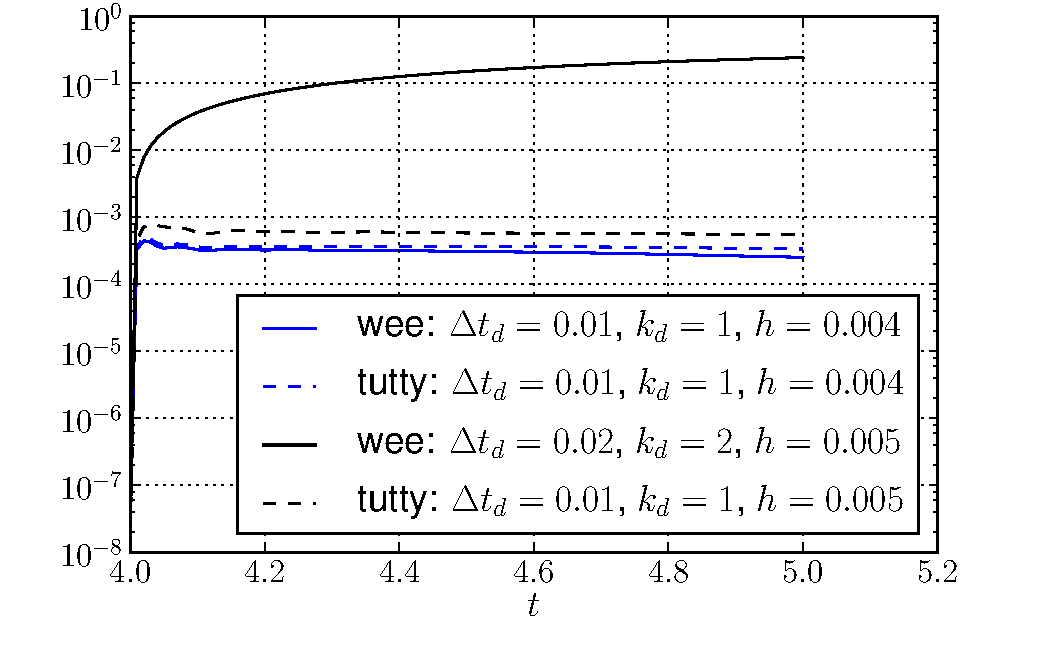
\includegraphics[width=0.6\textwidth]{figures/lagrangian/lambOseen_diffusionMethod_comparison_compressed.pdf}
	%	\caption{Comparison of Tutty's scheme TRS, and Wee-Ghoniem scheme WRS for treating diffusion. Figure depicts the growth in maximum relative error in vorticity, equation \ref{eq:maxRelErrorDef} from $t=0$ to $t=1$. 
	%	
	%	
	%	at $\Delta t_c = 0.01$. The Wee diffusion scheme with $\Delta t_d = \Delta t_c = 0.01$ [{\color{plotBlue}{---}}, solid blue], and $\Delta t_d = 2 \Delta t_c = 0.02$ [---, solid black]. The Tutty's diffusion scheme, $c^2 = 1/3$, with $\Delta t_d = \Delta t_c = 0.01$ [ {\color{plotBlue}{- -}}, dashed blue], and $\Delta t_d = \Delta t_c = 0.02$ [ - -, dashed black].}
	%	\label{fig:lambOseen_diffusionMethod_comparison_compressed}
	%	\end{figure}
	%	
	
  

%At $h = \num{4e-3}$, both schemes have the diffusion time step $\Delta t_d = 0.01$ meaning that the diffusion occurs at every iteration $k_d = 1$. During this time we see that the MRS performs slightly better that the SRS scheme. This is because, the diffusion of the vortex blobs is directly incorporated into the remeshing process, whereas the Tutty's SRS segregates the diffusion and the remeshing into two subsequent process. 

%At $h = \num{5e-3}$, the diffusion constraint on the Wee's MRS changes the minimum allowable diffusion time step to $\Delta t_d = 0.02$, meaning that diffusion has to be performs at every second step, $k_d=2$. Whereas for Tutty's SRS, we are not constraint by the minimum diffusion time step as so we can perform diffusion at $k_d = 1$. When investigating the growth in error for MRS, we see that the diffusion scheme has a large increase in the error, whereas the SRS does not have this limitation and is still able to diffuse at every step and has only a slight increase in error, figure \ref{fig:lambOseen_diffusionMethod_comparison_compressed} (solid black line). The diffusion scheme over-estimates the diffusion, and results in an incorrect diffusion process. However, we see that Tutty's SRS still performs a stable diffusion (dashed black line).

%This verification of the diffusion scheme showed that if Wee's MRS diffuses at $k_d > 1$, it will over-estimate the diffusion of the vorticity. Therefore, when using this scheme we will have to ensure that $k_d = 1$, by adjusting the convective time step appropriately. However, for large Reynolds number flows this is not possible, and so we must rely on the more stable and versatile Tutty's SRS diffusion scheme.

\subsection{Convergence study of the viscous vortex method}

Finally, we can perform a converge study, to validate that our scheme works according to the theory. For a scheme that is numerically stable, the error due to discretization must converge as the resolution of the discretization increases. 

	\begin{figure}[!b]
	        \centering
	        \begin{subfigure}[b]{0.5\textwidth}
	                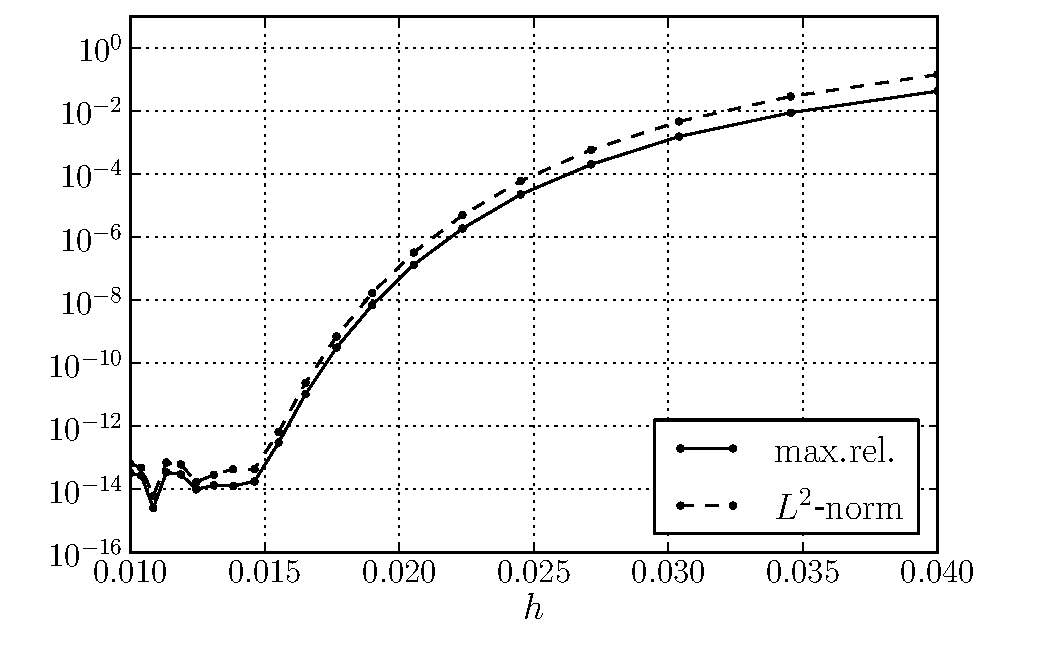
\includegraphics[width=\textwidth]{figures/lagrangian/lambOseen_convergence_dx_sigma0p02_compressed.pdf}
	                \caption{Error in vorticity vs. $h$ with $\sigma = 0.02$}
	                \label{fig:lambOseen_convergence_dx_sigma0p02_compressed}
	        \end{subfigure}%
	        ~ %add desired spacing between images, e. g. ~, \quad, \qquad etc.
	          %(or a blank line to force the subfigure onto a new line)
	        \begin{subfigure}[b]{0.5\textwidth}
	                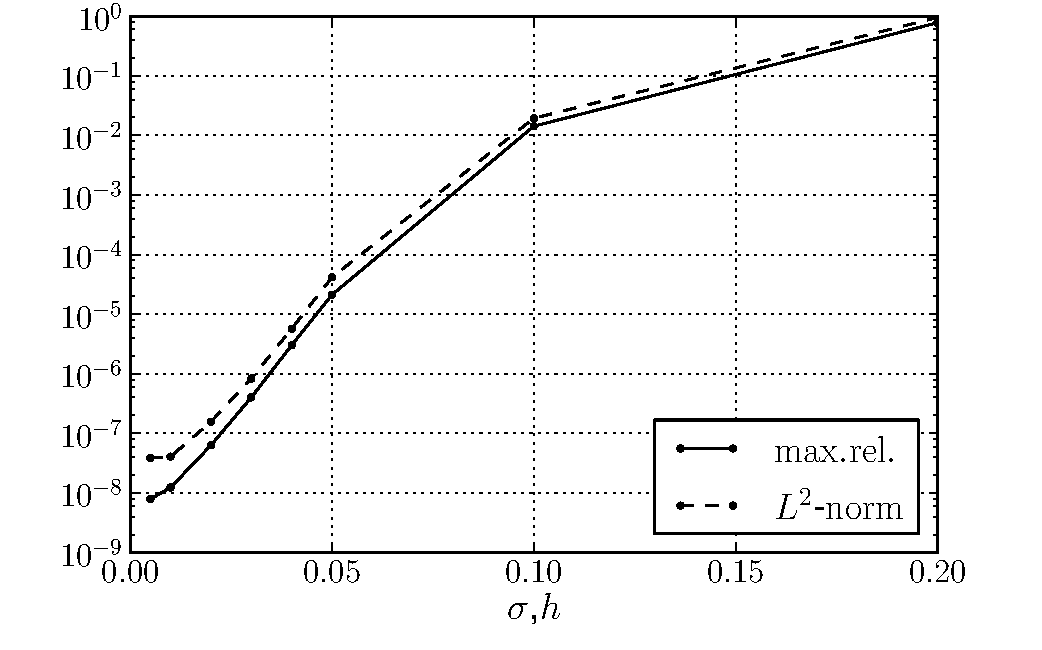
\includegraphics[width=\textwidth]{figures/lagrangian/lambOseen_convergence_dx_compressed.pdf}
	                \caption{Error in vorticity vs. $\sigma$, $h$ with $\lambda=h/\sigma=1$.}
	                \label{fig:lambOseen_convergence_dx_compressed}
	        \end{subfigure}
	        \caption{Convergence in spatial discretization of the vortex blobs. Figure \textbf{(a)} shows the convergence by fixing the core size $\sigma$ and \textbf{(b)} shows the convergence when overlap ratio $\lambda = h/\sigma = 1$.}
	        \label{fig:lambOseen_convergence_dx}
	\end{figure}

First, we investigate the convergence for spatial discretization. As we are dealing with vortex blobs, there are multiple ways of increasing the resolution. The straightforward method would be to increase the density of particles in a given area, i.e. reduce the blob spacing $h$ and maintaining the core spreading $\sigma$. Figure \ref{fig:lambOseen_convergence_dx_sigma0p02_compressed} shows the convergence of the spatial discretization when the core size $\sigma$ is maintained at $\sigma=0.02$. For this case, the overlap ratio changes with the blob spacing, described by equation \ref{eq:overlapRatio}. For small blob spacing $h$, the error in vorticity quickly drops to near machine precision. When investigating the order of convergence, we see that the error converges in a non-linear fashion and similar results have been obtained by Barba \cite{Barba2004c}.

Figure \ref{fig:lambOseen_convergence_dx_compressed}, shows the convergence of the error when the overlap ratio is fixed, $\lambda = 1$. In this test case, the core size scaled with the blob spacing, $h=\sigma$, and when increasing the spatial resolution, the error converges non-linearly.
	
	\begin{figure}[!h]
	\centering
	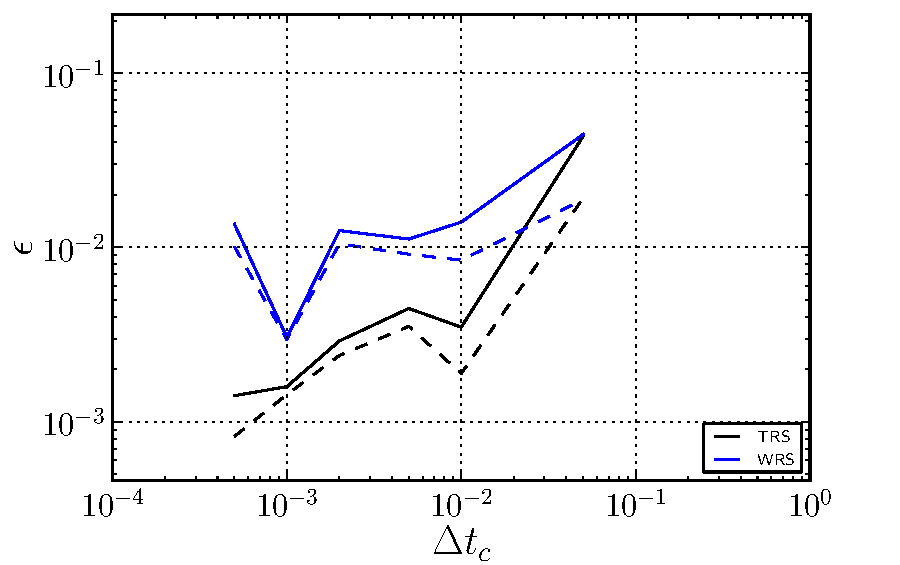
\includegraphics[width=0.6\textwidth]{figures/lagrangian/lambOseen_dtConvergence_WRSvsTRS.pdf}
	\caption{Convergence in temporal discretization of the vortex blobs. The Figure}
	\label{fig:lambOseen_dtConvergence_WRSvsTRS}
	\end{figure}	
	
To investigate the convergence in temporal discretization, we determined the evolution of the maximum relative error in vorticity, equation \ref{eq:maxRelErrorDef}, at $t=1$ for various convective time step sizes $\Delta t_c$, shown in figure \ref{fig:lambOseen_dtConvergence_WRSvsTRS}. At $t=1$, we see that the error reduces as we increase the temporal resolution meaning that we have a convergent scheme. We also observe that the error produced by WRS is higher than TRS and that it converges at a lower order than TRS. This again validates that TRS performs better than the WRS as it produces less error.


\section{Summary of the Lagrangian method}

In summary, we have investigated the Lagrangian domain of our hybrid method in this chapter. The Lagrangian method was used to described the evolution of the wake past the geometry. \printAcron{Vortex Particle Method}{VPM} was an ideal choice to describe the wake, as we require only to evolve the wake, and the generation of the vorticity is dealt with in the Eulerian domain. Unlike the Eulerian method, VPM only required the fluid elements where there was vorticity, meaning that the VPM was inherently auto-adaptive. Using the Population Control method, we were able to remove vortex blobs where they were not needed. Furthermore, the computation of the these elements were accelerated using an FMM, and simultaneously was parallelized using a GPU hardware. 

In section \ref{sec:introtovpm}, an introduction to the VPM was given. We determined advantage of the Lagrangian method w.r.t to the Eulerian method for resolving the wake for the VAWT. The velocity-vorticity formulation of the Navier-stokes equations is the governing equation of the VPM and we investigated the viscous splitting algorithm in section \ref{subsec:vsa}.

The viscous splitting algorithm enabled to perform diffusion and convection of the fluid is segregated steps. The discretization of the fluid through vortex blobs was investigated in section \ref{sec:spatialDiscretization}. These fluid elements has non-zero core size, removing the singularity when performing Biot-Savart calculations. 

In section \ref{subsec:vortexBlobInitialization}, we investigate the initialization of the vortex blobs. The proper initialization of the vortex blobs is a key factor for accurate coupling of Lagrangian method and the Eulerian method. The strengths of these particles is initialized by assigning the local circulation strength to the particle, as in equation \ref{eq:particleCirculationAssignment}. When the coupling is performed, it will be seen that the Gaussian blurring of the original vorticity field during the initialization is the fundamental source of error, section \ref{subsubsec:vfie}. Strategies such as Beale's iterative method, cannot be used as it is defined for an unbounded domain. The only approach found to minimize the Gaussian spreading initialization error is to increase the overlap ratio to $\lambda=1$, and minimize the blob spacing $h$ as much as possible, while keeping the computational effort to an acceptable level. The optimal strategy for the initialization of the vortex blob strengths is still an open question, and if solved can significantly improve the accuracy and the efficiency of the hybrid coupling

In section \ref{sec:covb}, we investigated the convection of the vortex blobs. The convection is performed using a $4^{\mathrm{th}}$-order Runge-Kutta time integration method. However, due to high strains in the fluid, the Lagrangian grid distortion of the vortex blob lattice has to be dealt with, section \ref{subsec:remeshing}. For this reason, we used a $\mathrm{M}'_4$ interpolation kernel that remeshed the particles onto a structured grid.

In section \ref{sec:diffusionVM}, we investigated two diffusion models for the vortex blobs. The WRS diffusion model developed by Wee and Ghonien \cite{Wee2006a}, integrated the diffusion process into the standard interpolation kernel.  This reduces computation cost, however the model was unfavourable constraint on the diffusion time step size, equation 
\ref{eq:la_dtcts}. The constraint limits the minimum diffusion step size and results in a discontinuous diffusion in time, as shown in figure \ref{fig:lambOseen_errorEvolution_WRSvsTRS_dt0p01}. To overcome this problem, we used the TRS diffusion model by Tutty \cite{Tutty2010a}, which enabled us to perform diffusion after every convection step, section
\ref{subsubsec:srs}. This also ensured that the diffusion process was continuous, which was important when performing the coupling algorithm.

In section \ref{sec:boundaryConditions}, we investigated the handling of the \emph{no-slip} boundary conditions for the viscous VPM. The boundary integral equations was used to enforces the wall boundary conditions in the Lagrangian method. We used the Constant-Strength Vortex panels, based on Katz \cite{Katz2001a}, to discretize the integral equations. The panel method was then verified and validated with the analytical solution of a potential flow around a cylinder in section \ref{sec:volm}. 

In section \ref{sec:volm}, we also verified and validated the implementation of the vortex blobs to analytical solution of the Lamb-Oseen vortex problem. We determined the evolution of the error for various spatial discretization and temporal discretization. The validation concluded that the implementation performed according to the literature, see example Barba \cite{Barba2004c}.



\section{Chapter Nomenclature}

{\textbf{\textsf{Latin Symbols}}}

{\renewcommand{\arraystretch}{1.2} %<- modify value to suit your needs
\begin{longtable}{p{1.5cm}p{10.5cm}p{1.5cm}}
    $\mathbf{A}$			& Vortex panel influence matrix						& -\\         

	$c^2$ 					& Diffusion parameter 								& - \\

    $\mathcal{E}$			& Enstrophy			  								& \si{m^2.s^{-2}} \\

	$f_{pc}$				& Population control frequency & - \\
	$f_{redis}$				& Redistribution frequency & - \\
	
    $h$						& Nominal particle spacing							& \si{m}\\   
    $h_{\nu}$				& Characteristic diffusion distance					& \si{m}\\ 

	$k$ & Gaussian kernel width spreading	& -\\
	$k_d$ & Frequency of vortex blob diffusion  								& -\\
    $\mathbf{K}$			& Biot-Savart kernel 								& -\\ 
    $\mathbf{K}_{\sigma}$	& Vortex blob kernel 								& -\\     

	$\hat{\mathbf{n}}$  	& Unit normal vector 								& -\\
	$N$  					& Number of vortex blobs (particles) 				& -\\

	$\lambda$			& Overlap ratio 									& - \\    
	
	$p$						& Pressure											& \si{Pa}\\

	$r$ 					& Radial position 									& \si{m}\\
	
	$\hat{\mathbf{s}}$		& Unit tangent vector								& - \\
	
	$t$						& Simulation time									& \si{s} \\
	
	$\mathbf{u}$			& Velocity 											& \si{m.s^{-1}}\\
	$\mathbf{u}_b$			& Velocity of the body 								& \si{m.s^{-1}}\\
	$\mathbf{u}_{\gamma}$	& Vortex sheet induced velocity                   	& \si{m.s^{-1}}\\	
	$\mathbf{u}_{\mathrm{ext}}$		& External induced velocity							& \si{m.s^{-1}}\\	
	$\mathbf{u}^h$			& Discrete velocity                               	& \si{m.s^{-1}}\\		
	$\mathbf{u}_{\infty}$	& Free-stream velocity								& \si{m.s^{-1}}\\			
	$\mathbf{u}_{\phi}$		& Free-stream velocity                            	& \si{m.s^{-1}}\\				
	$u_{r}$					& Radial velocity									& \si{m.s^{-1}}\\			
	$u_{\theta}$			& Angular velocity                               	& \si{m.s^{-1}}\\
	$\mathbf{u}_{\mathrm{slip}}$	& Boundary slip velocity					& \si{m.s^{-1}}\\
	$\mathbf{u}_{\omega}$	& Vorticity velocity 								& \si{m.s^{-1}}\\	

	$W$ 					& Interpolation kernel weight 						&-\\		
	$\mathbf{x}$			& Position vector 									& \si{m}\\		
	$\mathbf{x}_{\nu}$		& Position vector of particle to be diffused 		& \si{m}\\			
	$\mathbf{x}_{p}$		& Position vector of vortex blob (particle)			& \si{m}\\				
    %\caption{Attributes of \texttt{HybridSolver} class and their description.}
    %\label{tab:attributeHybrid}
\end{longtable}}

{\textbf{\textsf{Greek Symbols}}}

{\renewcommand{\arraystretch}{1.2} %<- modify value to suit your needs
\begin{longtable}{p{1.5cm}p{10.5cm}p{1.5cm}}
	$\alpha_p$ 		& Circulation of the particle & \si{m^2.s^{-1}}\\
	%$\beta_p$ 		& Corrected circulation of the particle & \si{m^2.s^{-1}}\\	

	$\Delta t_c$ 		& Convection time step size & \si{s}\\
	$\Delta t_d$ 		& Diffusion time step size & \si{s}\\	

	$\epsilon$ 		& Relative error & -\\		

	$\Gamma$ 		& Circulation & \si{m^2.s^{-1}}\\	
	$\Gamma_{glob}$ 		& Particle circulation threshold & \si{m^2.s^{-1}}\\	
	$\Gamma_{glob}$ 		& Total circulation threshold & \si{m^2.s^{-1}}\\		
	%$\Gamma_b$ 		& Circulation inside a moving body & \si{m^2.s^{-1}}\\		
	%$\gamma_c$ 		& Vortex sheet strength & \si{m^2.s^{-1}}\\			
	%$\Gamma_{\gamma}$ 	& Circulation of the vortex sheet & \si{m^2.s^{-1}}\\				
	%$\gamma_{\omega}$ 	& Circulation of the fluid & \si{m^2.s^{-1}}\\					

	$\nu$ & Kinematic viscosity & \si{m^2.s^{-1}}\\

	$\omega$ & Vorticity & \si{s^{-1}}\\
	$\tilde{\omega}$ & Vortex blob cell vorticity & \si{s^{-1}}\\
	$\omega^h$ & Discrete vorticity field & \si{s^{-1}}\\

	$\Omega$ & Fluid domain & \si{m}\\

	$\rho$ & Density & \si{kg.m^{-3}}\\
	
	$\sigma$ & Core size & \si{m}\\
	$\tau$ & Lamb-Oseen time constant & \si{s}\\
	$\xi$ & Scale relative position of particle to stencil node & -\\
	$\zeta_{\sigma}$		& Smooth cut-off function of the blobs & -\\			

\end{longtable}}

